\documentclass[ngerman,BCOR=4mm, english]{tudscrreprt}
\iftutex
  \usepackage{fontspec}
\else
  \usepackage[T1]{fontenc}
  \usepackage[ngerman=ngerman-x-latest]{hyphsubst}
\fi
\usepackage{babel}
\usepackage{isodate}
\usepackage{hyperref} % generate links to chapters etc.
\usepackage{mathtools}
\usepackage{graphicx} % for including graphics
\DeclarePairedDelimiter{\ceil}{\lceil}{\rceil} % for generating ceil over whole fraction
\DeclarePairedDelimiter{\floor}{\lfloor}{\rfloor}
% https://tex.stackexchange.com/questions/42271/floor-and-ceiling-functions#42274
\newcommand{\?}{\stackrel{?}{=}} % =? stacked symbol
\usepackage{microtype} % automatically fix overfull hboxes
\usepackage{xspace} % insert spacing after newcommands

% custom colors - TU Dresden colors
\usepackage{xcolor}
\definecolor{darkblue_tud}{RGB}{0,48,94}
\definecolor{blue_tud}{RGB}{0,106,179}
\definecolor{cyan_tud}{RGB}{0,158,224}
\definecolor{grey_tud}{RGB}{114,120,121}

% necessary to define concatenation-operator, because \parallel symbol doesn't work in tu dresden template
\DeclareMathOperator\concat{|\!\!|}

% drawing in latex
% https://tex.stackexchange.com/questions/241232/creating-dots-lines-brackets-in-tree-with-tikz
\usepackage{tikz}
%\usepackage{tikz-qtree} -> destroys current tikz-pictures, because changes arrow-tips
\usetikzlibrary{trees,calc,arrows.meta,positioning,decorations.pathreplacing,decorations.markings,bending}

\usepackage{forest} % forest library
%\usepackage{tikz-qtree}

% for highlighting python code - appendix, deprecated! 
%https://en.wikibooks.org/wiki/LaTeX/Source_Code_Listings
%\usepackage{listings} 
% for highlighting python code, not deprecated
\usepackage{minted}
\usepackage{scrhack} % fix: deprecated komascript warning

% package for multirows in tables
\usepackage{multirow}

% packages for pseudocode
% \usepackage{algorithm}
% \usepackage{algorithmic}

\newcommand{\extree}{T$_5$-Tree$^+$\xspace}
\newcommand{\tftree}{T$_5$-Tree\xspace}
\newcommand{\tfblock}{T$_5$-Block\xspace}
\newcommand{\tfblocks}{T$_5$-Blocks\xspace}
\newcommand{\tf}{T$_5$\xspace}

\begin{document}

\faculty{Faculty of Computer Science}
%\department{department?}
\institute{Institute of Systems Architecture}
\chair{Chair of Privacy and Security}
\date{09.03.2022}
\title{%
  Hash-based Digital Signature Schemes
}
\subject{master}
\graduation[M.Sc.]{Master of Science}
\author{%
  Amelie Wagner%
  \matriculationnumber{3949194}%
  \dateofbirth{17.09.1994}%
%  \placeofbirth{Dresden}%
}
%\matriculationyear{2010}
\supervisor{Dr.-Ing. Elke Franz \and M.Sc. Fabio Campos}
% \professor{Prof. Dr. ?}
%\makecover % add cover page
\maketitle % add actual title page 



\begin{otherlanguage}{ngerman} % selbstaendigkeitserklaerung deutsch
\confirmation
\end{otherlanguage}

\TUDoption{abstract}{true, notoc} % set header for abstract + don't show abstract in table of contents
\begin{abstract}
The security of current digital signature systems is in danger because they are not quantum secure. Hash-based digital signature schemes provide a good  countermeasure, but they generally perform worse in comparison to classical schemes. Therefore, performance improvement remains a crucial task.  
In this work, several state-of-the-art hash-based signature systems are analyzed in detail and methods for performance improvement are presented.
Using these methods, key generation is getting $25\%$ faster and signature verification up to $22\%$ faster. However, signature size is increased by up to $29\%$.
\end{abstract}

\tableofcontents
\chapter{Introduction}
\label{cha:introduction}
Attack examples on RSA: ~\cite{RSA_pq-attack_examples_2018}, \cite{RSA_pq-attack_without_factorization_2018}
% kurz: warum es post-quantum gibt/es  notwendig ist, quantum-threat, shors algorithm/grovers algorithm -> good source: https://dl.acm.org/doi/fullHtml/10.1145/3398388
% shors algo: \cite{shors_algo_original_1999}

% was gibt es: isogeniebasiert, hashbasiert, lattice, code usw
The common classes of quantum-secure cryptographic systems are as follows:~\cite{book_pqc_bernstein_2004}
\begin{enumerate}
\item Hash-based cryptography
\item Code-based cryptography
\item Lattice-based cryptography
\item Multivariate-quadratic-equations cryptography
\item Secret-key cryptography
\end{enumerate}

\section{Motivation}
% why signature systems 
% PQC threat -> RSA not safe anmyore 

% performance PQC Algos -> worse than "classic" ones
Comparison RSA/ECDSA with WOTS/MSS:
"The results showed that the two classical algorithms perform better in terms of the efficiency in key generation time, signature generation and verification time."~\cite{comparison_performance_RSA_ECDSA_Merkle_WOTS_2021}

% -> improve performance of PQC algorithm

\section{Goals}
% Analyze state of the art 
%Finding possible improvements to existing hashbased signature systems.
% Implement one improvement in existing algorithm

% T5 Paper hier bei Zielen -> Ziel ist Aufwand von Verfahren zu reduzieren, ohne Sicherheit zu beeinflussen
\chapter{Background}
\label{cha:background}
This chapter addresses the scientific background needed for this work. First, the general concept of digital signature systems and hash functions are elaborated. Afterwards, the most common concepts for hash-based digital signature systems are explained. The presented hash-based schemes are the \textit{Lamport-Diffie one-time signature scheme~(LD-OTS)}, the \textit{Winternitz one-time signature scheme~(W-OTS)}, the \textit{Merkle signature scheme~(MSS)} and the \textit{extended Merkle signature scheme~(XMSS)}.

\section{Digital Signature Schemes}
% ! digital signature scheme -> assymetris ch (immer?) 
A \textit{digital signature scheme} uses a set of rules and a set of parameters to verify the identity of the originator, the integrity of data and non-repudiation.~\cite{cha:bg_digital_sign_schemes_NIST_standard1992} 
% Non-repudiation: It prevents an entity from denying previous commitments or actions.
% Integrity: Guarding against improper information modification or destruction, and includes ensuring information non-repudiation and authenticity -> https://nvlpubs.nist.gov/nistpubs/Legacy/SP/nistspecialpublication800-18r1.pdf
% -> desrcibe in table/more specific, what integrity/non-repudiation/etc. means
% -> description already in the following textblock, maybe put in table for overview?

In this section, for explanatory reasons, data refers to a message being sent from one sender to a recipient across a network (e.g. LAN). The sender is the person signing the message, the recipient usually wants to verify the received message, therefore they are referred to as signer and verifier. Notably, the verifier can also be a third party, not just the recipient.
The \textit{digital signature~$\sigma$} of a message, generated by a digital signature scheme, is a value dependent on some secret known only to the signer (usually the private key~$X$) and on the content of the message being signed. With the corresponding public key~$Y$ (without having access to the signer's private key $X$) the authenticity of the signature can be verified: It is ensured that the message actually belongs to the signer - e.g. a lying signer trying to repudiate their signature, a fraudulent claimant arguing the message is theirs, or a message that has been tampered with can be detected.
% hier vlt Bild von Signatursystem?
% hier schutzziele erwähnen (vlt Liste?) -> recipient will bestätigung das nachricht wirklich vom empfänger, sender will dass recipient ihm keine falschen nachrichten unterschiebt -> oder Schutzziele schon im 1. Satz
To ensure the above mentioned properties of digital signatures, a digital signature scheme consists of the following parts (see also Figure~\ref{img:digital_sign_system_simple}):~\cite{cha:bg_signature_schemes_book_menezes2018_1997} % gehört keygen wirklich zu signatursystem? -> ganze section beruht auf diesem Buch, wird das klar?

\begin{figure}
\centering
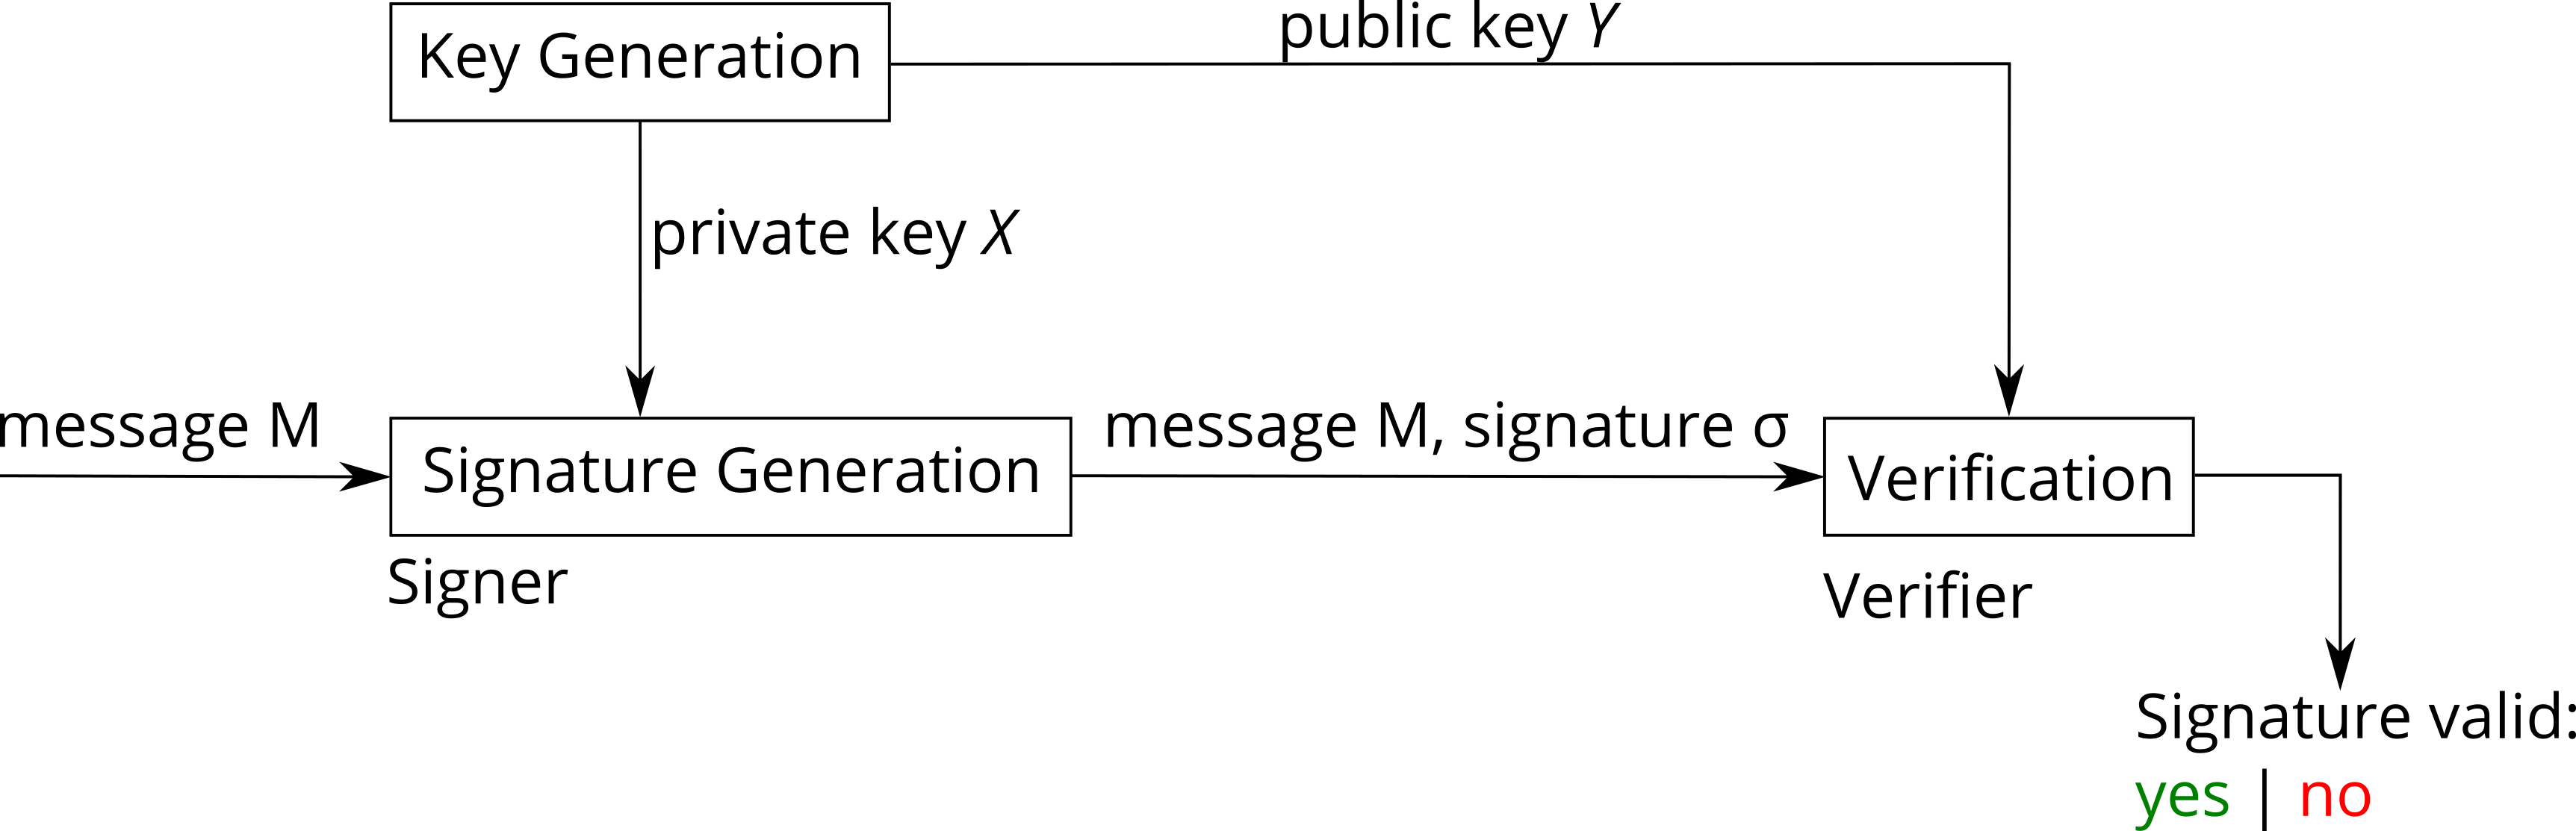
\includegraphics[width=\linewidth]{images/Background/Digital_Signaturesystem_Simple.png}
\caption{The general structure of a digital signature system. %Elke: Nur den ersten Satz als caption. Das hier nicht: The key generation algorithm creates the private key~$X$ and public key~$Y$, whereas $X$ is only known to the signer and $Y$ is made public for the verifier. The signer creates the message $M$ and signs it with the private key, using the signature generation algorithm. Afterwards, the so generated signature~$\sigma$ and the corresponding message~$M$ are sent to the verifier. The verifier checks the validity of the message and the corresponding signature with the public key (that is already known after key generation and distribution) and the verification algorithm. If the verification algorithm evaluates returns a valid result, the verifier can trust the message or otherwise knows it has been tempered with).
}
\label{img:digital_sign_system_simple}
\end{figure} 

\begin{enumerate}
\item The \textit{key generation algorithm} creates a private key~$X$ used for signature generation, and a public key $Y$ used by the recipient for signature verification. Both keys are mathematically dependent from each other, in which way is determined by the specific type of signature scheme (e.g. the Winternitz signature scheme, see Section~\ref{sec:WOTS_keygen}). % und auch noch von weiteren Leuten die Originalität von Nachricht prüfen wollen? Aber in meinem runtergebrochenen Beispiel nur 2 Leute, außerdem wird nicht erklärt dass auch key signiert wird
\item The \textit{signing algorithm} creates the digital signature~$\sigma$ of a message dependent on the private key $X$ of the signer and the content of the message.
\item The \textit{verification algorithm} is used by the verifier to check the validity of the signature~$\sigma$ and the corresponding message with the public key $Y$.
\end{enumerate}
% Y muss vor signieren der Nachricht veröffentlich werden

% Bild / Schema einfügen

% es wird message digest signiert
% Überleitung zu Hashfunctions

\section{Definition of Hash Functions} 
\label{sec:def_hashfunctions}
The security of the following presented \textit{One-Time Signature Schemes} (see section~\ref{sec:one-time_sign_schemes}) %Elke: Man könnte auch sagen, dass Signaturverfahren i. Allg. Hashfunktionen verwenden ...
is based on cryptographic secure hash functions. A hash function is a function that can be computed efficiently and maps strings of arbitrary length to strings of fixed length~\cite{cha:bg_hashfunctions_thesis_matusiewicz2007}. Therefore, a hash function $h$ is defined as any function $h$ with arbitrary length input to a fixed length output: $h: \{0,1\}^* \rightarrow \{0,1\}^n$~\cite{cha:bg_hashfunctoins_Stinson2006}. A hash function is considered \textit{cryptographically secure} if it has the following  properties:~\cite{cha:bg_hashfunctions_BASIC_DEFINITIONS_Springer2004} 

\begin{enumerate} % vlt: ? -> in x umbenennen in Zeichnungen + x in text auch blau machen damit klar ist, dass es das gesuchte ist
	\item \textbf{Preimage-Resistance / One-wayness}
	 A hash function $h$ is preimage-resistant if given an output value $y$, it is computationally infeasible to find any input which generates this output, i.e. finding any preimage $x$ such that $h(x) = y $ (when given any $y$). 

\begin{minipage}[t]{.5\linewidth}
          	\raggedright
            
\includegraphics[width=.8\linewidth]{images/Background/preimage_res_horizontal.png}
	      \end{minipage} 

	\item \textbf{Second Preimage-Resistance}
	A hash function $h$ is second preimage-resistant, if given any input value and the corresponding output, it is computationally infeasible to find another distinct
input that produces the same output, i.e. given any $x$ finding a second preimage $x \neq x'$ such that $h(x) = h(x')$. % oder erst formel -> dann beschreibung dran?

\begin{minipage}[t]{.6\linewidth}
          	\raggedright
            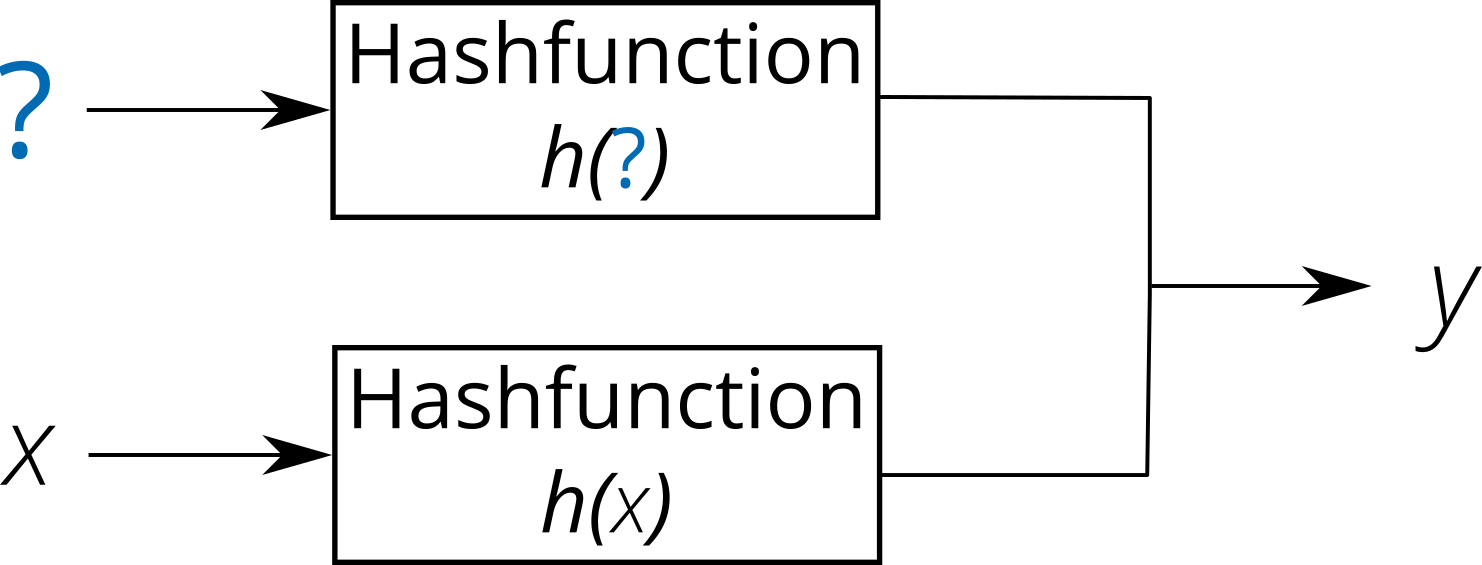
\includegraphics[width=.8\linewidth]{images/Background/second_preimage_res_horizontal.png}
	      \end{minipage} 
	
	\item \textbf{Collision Resistance}
	A hash function $h$ is called collision-resistant, if it is computationally infeasible to find a pair of different inputs $x, x'$ that map to the same output value, such that $h(x) = h(x')$.


\begin{minipage}[t]{.6\linewidth}
          	\raggedright
            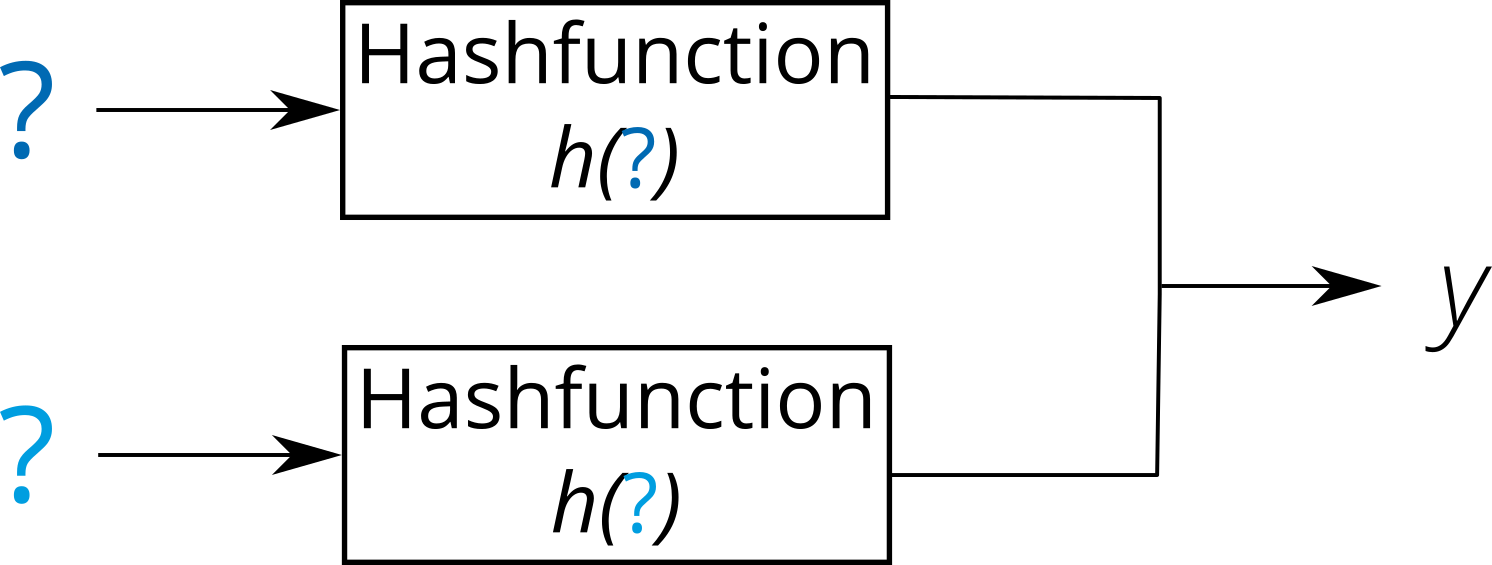
\includegraphics[width=.8\linewidth]{images/Background/collission_res_horizontal.png}
	      \end{minipage}
	      
\end{enumerate}	      


\section{One-Time Signature Schemes}
\label{sec:one-time_sign_schemes}
This section is based on the work of Buchmann et al~\cite{book_pqc_bernstein_2004}. 
% ONE-Time Signature scheme anmerken / erklären
The two signature schemes Lamport-Diffe and Winternitz are both \textit{one-time signature schemes (OTS)}, meaning the public and private key can be used \textbf{once}, for signing a single message. If they are used for generating more than one signature, the signature can be forged. % vlt rauslöschen einfach
The following types of functions are used for the Lamport-Diffie One-Time Signature Scheme and the Winternitz One-Time Signature Scheme: 
The cryptographic hash function~$h$ is preimage resistant, second preimage-resistant and collision resistant, it is applied to the original message and generates the message digest.
The one-way function~$f$ is a hash function that is at least preimage-resistant and takes a fixed input length, because it is applied to the message digest.% später wird Benutzung von h und f noch sichtbar
% hier erklären was one time signature scheme ist & dass LD-OTS und Winternitz-OTS erklärt werden

\begin{equation}
\label{eq:basic_hashfunc}
\textbf{Cryptographic hash function h: } \lbrace 0,1 \rbrace^* \rightarrow \lbrace 0,1 \rbrace^n
\end{equation}

\begin{equation}
\label{eq:one-way-func}
\textbf{One-way function f: } \lbrace 0,1 \rbrace^n \rightarrow \lbrace 0,1 \rbrace ^n
\end{equation}


\subsection{Lamport-Diffie One-Time Signature Scheme (LD-OTS)}
The Lamport–Diffie one-time signature scheme (LD-OTS) was first proposed by Leslie Lamport in 1979~\cite{lamport_signature_scheme_1979}. 

\subsubsection{LD-OTS Key Generation}
The private key X consists of $2n$ bit strings, each of length $n$, chosen at random. As the key size and signature size are dependent on $n$, it is also referred to as security parameter.
% n ist security parameter
% !! einfügen, was n für eine Rolle spielt

\begin{equation}
\label{eq:ldots_sign_key}
X = \left(x_{0}\left[0\right], x_{0}\left[1\right], x_{1}\left[0\right], x_{1}\left[1\right], \cdots, x_{n-1}\left[0\right], x_{n-1}\left[1\right] \right)
\end{equation}
The public key $Y$ is created out of the private key $X$. For each $x_i[j] \in X, 0 \leq i \leq n-1, j \in \lbrace 0,1 \rbrace$, the one-way function~f (see Equation~\ref{eq:one-way-func}) is applied.

\begin{equation}
y_i[j] \in Y = f(x_i[j]), 0 \leq i \leq n-1, j \in \lbrace 0,1 \rbrace
\end{equation}

\begin{equation}
Y = \left( 
y_{0}\left[0\right], y_{0}\left[1 \right], y_{1}\left[0\right], y_{1}\left[1\right], \cdots, y_{n-1}\left[0\right], y_{n-1}\left[1\right]
\right)
\end{equation}

\subsubsection{LD-OTS Signature Generation} % m has fixed length
Before signing, the public key $Y$ has to be published.
The private key $X$ (see Equation~\ref{eq:ldots_sign_key}) is used to sign the message $M \in \lbrace 0,1 \rbrace^*$. 
The cryptographic hash function $h$ (see Equation~\ref{eq:basic_hashfunc}) is applied to $M$ in order to get the hash digest $m$ of fixed length $n$.

\begin{equation}
\label{eq:hash_message}
m = h(M) = (h_{0}, \cdots, h_{n-1})
\end{equation} % Elemente von m ENTWEDER m_i ODER h_i
For each bit $h_i \in m$, the corresponding $x_i[h_i]$ out of private key $X$ is chosen, resulting in signature $\sigma$ for message $m$.
% h_i in m_i umbenennen oder umgekehrt -> konsequent bleiben
\begin{equation}
\sigma = \left(
x_0 \left[ h_0 \right], x_1\left[ h_1 \right], \cdots, x_{n-1}\left[ h_{n-1}\right]
\right) = (\sigma_0, \cdots, \sigma_{n-1})
\end{equation}

\subsubsection{LD-OTS Verification}
After receiving a message $M$ with the corresponding signature $\sigma$, the verifier calculates the message digest $h(M) = m$. 
To verify the given signature $\sigma$, it is necessary to check the following condition.
\begin{equation}
\left(
f(\sigma_0), \cdots, f(\sigma_{n-1})
\right) =
\left(
y_0[h_0], \cdots, y_{n-1}[h_{n-1}]
\right)
\end{equation}
If the condition is true, the signature is valid.

% nochmal extra auf Einmalverwendung hinweisen
% table with properties i.e.
% keygen+sign+verify time / aufwand / speicherverbrauch -> Positiv: schnelle signatur+keygen Negativ: Viel Speicherverbrauch
% Überleitung zu Winternitz weil diese Vorteil kürzerer Signatur aufweisen

\subsection{Winternitz One-Time Signature Scheme (W-OTS)}
\label{sec:wots_general}
LD-OTS signatures are efficient to calculate but have a huge size. % somewhere else explain that huge signature -> need much "memory"-> bad ? or is it obvious
The Winternitz one-time signature scheme (W-OTS) generates signatures with substantially shorter size. W-OTS uses the same hash function (Equation~\ref{eq:basic_hashfunc}) and one-way function (Equation~\ref{eq:one-way-func}) as LD-OTS. %genauer beschreiben evtl

\subsubsection{W-OTS Key Generation}
\label{sec:WOTS_keygen}
First, two parameters are selected: The Winternitz-Parameter $w \geq 2$ and the security parameter $n$. As $n$ is the length of the message digest, increasing it leads to higher security because it increases the collision resistance of the hash function. The Winternitz parameter $w$ enables space/time trade-offs, for a detailed explanation see end of Section~\ref{sec:wots-verification}/W-OTS Verification.

After selecting the parameters $w$ and $n$, the values $t_1, t_2, t$ are calculated.
The value $t_1$ determines the amount of blocks the message digest $m$ will be separated into (see Equation~\ref{eq:hash_digest_split}):
\begin{equation}
\label{eq:t1}
t_1 = \ceil[\Bigg]{\frac{n}{w}}
\end{equation}
The value $t_2$ determines the amount of blocks the checksum $c$ will be separated into (see also Equation~\ref{eq:checksum_calculation}):
\begin{equation}
\label{eq:t2}
t_2 = \ceil*{\frac{\floor*{\log_2 t_1} + 1 + w}{w} }
\end{equation}
The value $t$ determines the total amount of blocks (see Equation~\ref{eq:block_B_out_of_M_and_C}) as well as the amount of elements in the private/public key (see Equation~\ref{eq:wots_privkey},\ref{eq:wots-generation-one-time-public-key}) and the signature (see Equation~\ref{eq:wots_sign_calc}):
\begin{equation}
\label{eq:t}
t = t_1 + t_2
\end{equation}
The private key $X$ consists of $t$ bit strings, each of length $n$ chosen at random.
\begin{equation}
\label{eq:wots_privkey}
X = (x_0, \cdots, x_{t-1})
\end{equation}
The public key $Y$ is generated by applying the one-way function~$f$ to each element $x_i  \in X$  consecutively $2^w - 1$ times. % hier sieht man dass höheres w -> höherer Aufwand Keygen
\begin{equation}
\label{eq:wots-generation-one-time-public-key}
y_i \in Y =  f^{2^w-1}(x_i), 0 \leq i \leq t-1 
\end{equation}

\begin{equation}
Y = (y_0, \cdots, y_{t-1})
\end{equation}
Each $y_i \in Y$ is a bit string of length $n$. The public key $Y$ has to be published before the signature can be generated. One value of the public key is corresponding to one full \textit{Winternitz chain}. % maybe introduce Winternitz chain another way?

\subsubsection{W-OTS Signature Generation}
For signing a message $M \in \lbrace 0,1 \rbrace^*$, the cryptographic hash function~h (see Equation~\ref{eq:basic_hashfunc}) is applied to $M$ (see Equation~\ref{eq:hash_message}). The resulting hash digest $m$ is split into $t_1$ bitstrings of length $w$. If $m$ is not divisible by $w$, it is necessary to add leading zeros to $m$ before splitting.

\begin{equation}
\label{eq:hash_digest_split}
m = m_0 \concat m_1 \concat \cdots \concat m_{t_1-1}
\end{equation}
Each bitstring $m_i \in m$ is converted to its decimal representation in order to calculate the checksum $c$. A detailed example why the checksum is necessary is shown at section~\ref{sec:checksum_explained}. % ! reference to subsubsection doesn't work: https://tex.stackexchange.com/questions/198800/how-to-number-and-cross-reference-subsubsection-level-headers and https://blog.chapagain.com.np/latex-numbering-subsubsection-and-showing-it-in-table-of-contents/

\begin{equation}
\label{eq:checksum_calculation}
c = \sum_{i = 0}^{t_{1}-1}(2^w-m_i)
\end{equation}
The checksum $c$ is divided into $t_2$ bitstrings of length $w$. In order to divide $c$ this way, it can be necessary to add leading zeros to $c$ as a padding.
\begin{equation}
c = c_0 \concat c_1 \concat \cdots \concat c_{t_2 - 1}
\end{equation}
Afterwards, $m$ and $c$ are concatenated to one block~$B$. This leads to $t$ bitstrings of length $w$ in total, as $t = t_1 + t_2$.

\begin{align}
\label{eq:block_B_out_of_M_and_C}
B &= m \concat c  \\ 
&= m_0 \concat \cdots \concat m_{t_1 - 1} \concat c_0 \concat \cdots \concat c_{t_2 - 1} \nonumber \\
&= b_0 \concat \cdots \concat b_{t-1} \nonumber
\end{align}
The signature $\sigma$ is calculated by applying the one-way function~$f$ to each part of the private key $X$ (see Equation~\ref{eq:wots_privkey}) several times: The element $b_i \in B$ determines the amount of times the hash function $f$ is applied to the corresponding $x_i \in X$. One element of the signature is also referred to as one \textit{Winternitz chain}.

\begin{equation}
\label{eq:wots_sign_calc}
\sigma = (f^{b_0}(x_0), f^{b_1}(x_1), \cdots, f^{b_{t-1}}(x_{t-1})) = (\sigma_0, \cdots, \sigma_{t-1})
\end{equation}

\subsubsection{W-OTS Verification}
\label{sec:wots-verification}
Given a signature $\sigma$ and message $M$, the hash digest $m$ is generated (see Equation~\ref{eq:hash_message}). Afterwards, the block $B$ is generated out of~$m$ as shown in the previous section (see Equations~\ref{eq:hash_digest_split} to~\ref{eq:block_B_out_of_M_and_C}). To check if the given signature is valid, the one-way function~$f$ is applied $2^w - 1 - b_i$ times to each $\sigma_i \in \sigma$. The result is compared to the corresponding $y_i \in Y$. This can also be described as advancing each Winternitz chain in the signature by applying~$f$, until the  values of the public key are reached.

\begin{equation}
(f^{(2^w-1)-b_0}(\sigma_0), \cdots, f^{(2^w - 1) - b_{t-1}}(\sigma_{t-1})) \? (y_0, \cdots, y_{t-1})
\end{equation}
If each $f^{2^w-1-b_i}(\sigma_i) = y_i$, the signature is valid because $\sigma_i = f^{b_i}(x_i)$ and therefore

\begin{gather}
f^{2^w-1-b_i}(\sigma_i) = f^{2^w-1}(x_i) = y_i \\
0 \leq i \leq t-1 \nonumber
\end{gather}
As $w$ determines the block size of each block in $B$, $w$ is allowing a space/time trade-off: When increasing $w$, the signature size will decrease linearly (the total amount of blocks in $B$ will decrease) and the effort for key generation, signing and verification will increase exponentially (because $w-1$ hash function calls are necessary for public key generation, and $w-1$ hash function calls are necessary for signature generation+verification in total).

\subsubsection{W-OTS Example Calculation}
\label{sec:w-ots_example_calc}
This section contains an example calculation of W-OTS, including key generation, signature generation, and signature verification.
% ! explain that example one-way function is not cryptographic secure, is only example

\begin{enumerate}

\item The first step is choosing the following parameters:
$n=3, w=2, \text{message digest } m = 101, {\text{one-way function } f:\{0,1\}^{3} \rightarrow \{0,1\}^{3}, x \rightarrow x+2 \text{ mod } 8}$

% ceilings of t_2 are a bit ugly. Maybe fix later
\item Calculating $t_1, t_2, t$: \\
$t_1 = \ceil{\frac{n}{w}} = \ceil{\frac{3}{2}} = 2, t_2 = \ceil*{\frac{\floor*{\log_2 t_1} + 1 + w}{w} } = \ceil*{\frac{\floor*{\log_2 2} + 1 + 2}{2} } = 2, {t = t_1 + t_2 = 2+2 = 4}$

\item Choosing the private key $X$ with $t=4$ random bit strings of length $n=3$: \\
$X = (x_0, \cdots, x_{t-1}) = (x_0, x_1, x_2, x_3) = 
\begin{psmallmatrix}
1 & 1 & 0 & 1\\
0 & 1 & 1 & 1\\
1 & 1 & 1 & 0
\end{psmallmatrix} \in \{0,1\}^{(3,4)} $

\item Calculating the public key $Y$ from $X$ by applying $f$ to each element in $X$ for $2^w-1 = 3$ times:	
$Y = (y_0, \cdots, y_{t-1}) = (y_0, y_1, y_2, y_3) = 
\begin{psmallmatrix}
0 & 1 & 0 & 1 \\
1 & 0 & 0 & 0 \\
1 & 1 & 1 & 0
\end{psmallmatrix} \in \{0,1\}^{(3,4)} $ 

\item To make $m$ divisible by $w$, a leading zero is inserted. Then it is split in blocks of length $w$: $m = 01 \concat 01 = m_0 \concat m_1$. These blocks are used for the checksum calculation: \\ $c = (2^w - m_0) + (2^w - m_1) = (4-1)+(4-1)=6$. To make $c$ divisible by $w$ as well, one leading zero is added to the binary representation of $c$. Then, splitting $c$ in blocks of length $w$ yields $c = 01 \concat 10 = c_0 \concat c_1$.

\item The block $B$ is generated by concatenating $m$ and $c$: \\ $B = m_0 \concat m_1 \concat c_0 \concat c_1 = b_0 \concat b_1 \concat b_2 \concat b_3 = 01 \concat 01 \concat 01 \concat 10 $.

\item %The signature $\sigma$ is created by applying $f$ to each element in $X$.
%The block $B$ determines the amount of applying $f$ to $X$
The signature $\sigma$ of $m$ is determined by the parameter $B$ and one-way function $f$: \\ % hier besser erklären dass man dezimalrepr. von B und X nimmt?
$\sigma = (f^{b_0}(x_0), f^{b_1}(x_1),f^{b_2}(x_2),f^{b_3}(x_3)) = (f^1(5),f^1(7),f^1(3),f^2(6)) = (\sigma_0, \sigma_1, \sigma_2, \sigma_3) = \\
\begin{psmallmatrix}
1 & 0 & 1 & 0 \\
1 & 0 & 0 & 1 \\
1 & 1 & 1 & 0
\end{psmallmatrix} \in \{0,1\}^{(3,4)} $

\item The verifier knows $Y, w, n$ and therefore $t_1, t_2$ and $t$. After receiving $m, \sigma$ from the signer, the block $B$ is calculated as explained in the previous steps. The validity of the signature $\sigma$ is checked by calculating: \\
$( f^{2^w-1-b_0}(\sigma_0), f^{2^w-1-b_1}(\sigma_1), f^{2^w-1-b_2}(\sigma_2), f^{2^w-1-b_3}(\sigma_3)) = (f^2(7) , f^2(1), f^2(5), f^1(2)) = \\ \begin{psmallmatrix}
0 & 1 & 0 & 1 \\
1 & 0 & 0 & 0 \\
1 & 1 & 1 & 0
\end{psmallmatrix} \in \{0,1\}^{(3,4)} $
\\ Because these values are the same as in the public key $Y$, $\sigma$ is valid. 

\end{enumerate}

\subsubsection{W-OTS Checksum Example}
\label{sec:checksum_explained}
In this section, the necessity of the W-OTS checksum (see also Equation~\ref{eq:checksum_calculation}) is explained with an example. 
The attack prevented by the checksum is an \textit{adaptive chosen-message attack}: It is possible for the attacker to generate new messages with matching signatures which depend on previously obtained signatures and messages~\cite{cha:bg_signature_schemes_book_menezes2018_1997}. 
After obtaining a message and corresponding signature, the idea behind the attack is to increase the bits of the received message to generate a new message. The hash function is applied respectively to the corresponding digits in the signature, increasing the Winternitz chain. Then, without the checksum, a new valid signature would be generated for the message. For this example, the same parameters for W-OTS are used as in the the section before. % (see section~\ref{sec:w-ots_example_calc}. again_: need correct subsubsection label

\begin{enumerate}
\item We assume the attacker knows the message digest $m = 101$, the corresponding signature $\sigma = (\sigma_0, \sigma_1, \sigma_2, \sigma_3)$ and the parameters $w=2, n=3, Y, f$ of the example in the section before. The attacker can get this information because a digital signature system does not ensure confidentiality of the message or the parameters, the premise is the secrecy of the private key. The goal of the attacker is to forge a signature $\sigma' = (\sigma_0', \sigma_1', \sigma_2', \sigma_3')$ to get a valid signature for a message $m'$ chosen by the attacker. 
% (e.g. the attacker was also the receiver of the message or intercepted the channel where the message was sent)

\item The attacker calculates $m  = m_0 \concat m_1 = 01 \concat 01$, $c = c_0 \concat c_1 = 01 \concat 10$ and therefore $B =  b_0 \concat b_1 \concat b_2 \concat b_3 = 01 \concat 01 \concat 01 \concat 10$ (see steps 1-6 in section before).

\item The original message $m = 101$ is increased by one: $m' = 111$. Make $m'$ divisible by $w = 2$, insert leading zero: $m' = m_0'\concat m_1' = 01 \concat 11$. Calculate checksum $c' = (2^w - m_0') + (2^w - m_1') = (4-1)+(4-3)=4$.
Insert leading zero to $c'$ to make it divisible by $w$: $c' = c_0' \concat c_1' = 01 \concat 00$. Therefore, $B' = b_0' \concat b_1' \concat b_2' \concat b_3' = 01 \concat 11 \concat 01 \concat 00$.

Now, the attacker can forge $\sigma_0', \sigma_1'$ of the signature $\sigma'$:
As $b_0 = b_0' = 01$, $\sigma_0' = \sigma_0$.
Because the difference between $b_1 = 01$ and $b_1' = 11$ is $2$, applying $f$ two more times to $\sigma_1$ leads to $\sigma_1'$: $f^2(\sigma_1) = \sigma_1'$.

Notably, $\sigma_0, \sigma_1$ depend only on the message bits $m_0, m_1$, not on the checksum. Therefore, the attacker could forge a signature for $m'$ without the checksum. But because of the checksum bit $c_3 = b_3 = 10, c_3' = b_3' = 00$, $b_3 > b_3'$, it is not possible to calculate $\sigma_3$: The attacker would have to calculate $f^{-2}(\sigma_3)$, that is finding two times a preimage to $\sigma_3$. As long as the hash function $f$ is preimage resistant, which is assumed (see also Equation~\ref{eq:one-way-func}), this is not possible. The attacker can not forge the complete signature $\sigma'$.

\end{enumerate}
For a general proof of security of the checksum, see Section 9.3 in McGrew et al.~\cite{LMS_RFC8554}.
For LD-OTS, the checksum is not necessary because only one hash function call is used to get to the public key $Y$. Therefore, it is not possible to generate another valid signature $\sigma'$ by applying the hash function to the known signature $\sigma$ again.

%For a general proof, see https://datatracker.ietf.org/doc/html/rfc8554#section-9.3

% Why checksum is necessary: This checksum is needed because an attacker can freely advance any of the Winternitz chains.  That is, if this checksum were not present, then an attacker who could find a hash that has every digit larger than the valid hash could replace it (and adjust the Winternitz chains).-> citation: RFC of LMS (https://www.rfc-editor.org/rfc/rfc8554.html#section-4)
% genaue beschreibung checksum bsp angriff: https://datatracker.ietf.org/doc/html/rfc8554#section-9.3
% https://crypto.stackexchange.com/questions/31696/winternitz-signature-in-standard-model -> stackoverflow frage + antwort genau dazu

\section{Merkle Signature Scheme (MSS)} 
\label{sec:mss}
%!! Zitierung fehlt von Buchmann
The main disadvantage of the one-time signature schemes introduced in Section~\ref{sec:one-time_sign_schemes} is the restriction to use each key pair (consisting of private key~$X$ and public key~$Y$) for only one signature. This is inadequate for most practical situations, because the key generation as well as the key distribution take a lot of time and effort that could be saved otherwise.
To solve this problem, Merkle~\cite{cha:bg_merkletrees_Merkle_1979} proposed the concept of using a binary hash tree, where each leaf represents a different one-time key pair, the \textit{Merkle Signature Scheme (MSS)}. The root of the tree is the public key $Y_{MSS}$  which combines the one-time key pairs at the leafs. With a tree depth $d$, $2^d$ one-time key pairs and corresponding signatures can be generated. % achtung: bei RSA mehr, possibly unendlich
This concept is denoted as \textit{Merkle signature scheme (MSS)} and it works with any cryptographic hash function and any one-time signature scheme. 
The structure of the Winternitz one-time signature scheme fits better into MSS than the Lamport-Diffie one-time signature scheme: When using W-OTS, it is not necessary for the signer to put the public one-time signature key $Y_s$ in the one-time signature $\sigma_s$. The verifier will automatically calculate $Y_s$ from the given one-time signature. Therefore, the chosen one-time signature scheme for MSS in this chapter is W-OTS. The cryptographic hash function~$h$ (see Equation~\ref{eq:basic_hashfunc}) is used. 
% Moreover, when using LD-OTS: All X_s (for signature) + corresponding Y_s are needed. Not enough when verifier knows only the X_s that are needed for OTS-signature, moreover the rest of Y_s are needed (because all "leaves" are needed) to build the merkle tree.

\subsection{MSS Key Generation}
\label{cha:mss_keygen}
For a depiction of the Merkle tree referenced in this section, see Figure~\ref{img:merkle_tree}.
The signer chooses the tree depth~$d$ where $d \geq 2$, and generates $2^d$ one-time key pairs $(X_j, Y_j)$ where $0 \leq j \leq 2^d-1$, with $X_j$ being the private key and $Y_j$ the corresponding public key. The \textit{leaves} of the Merkle tree are the hash digests $H_{i,j}$ of the public key $Y_j$.
\begin{gather}
\label{eq:leaf_merkle_tree:hash_digest_publ_key_Y}
H_{i,j} = h(Y_j) \\ 
0 \leq j \leq 2^d - 1 \nonumber
\end{gather}
The \textit{inner nodes} of the Merkle tree are computed as follows: Each parent node $H_{i,j}$ is the hash digest of the concatenation of its direct two children: % $H_{i+1,j}$ and $H_{i+1,j+1}$.

% ! wichtig dass 0 <= i < d weil Blätter zählen nicht mit
\begin{gather}
\label{eq:inner_nodes_merkle_tree_keygen}
H_{i,j} = h(H_{i-1,2j} \concat H_{i-1,2j+1}) \\
1 \leq i \leq d \nonumber \\ 
0 \leq j < 2^{d - i} \nonumber
\end{gather} 
The \textit{root} of the Merkle tree is the MSS public key~$Y_{MSS}$. The MSS private key~$X_{MSS}$ is the collection of one-time signature keys generated before constructing the Merkle tree.
% Y_mss = H_d,0 because d=height of tree
\begin{align}
\label{eq:mss_priv_key}
X_{MSS} &= (X_0, \cdots, X_j, \cdots, X_{2^d - 1} ) \\
Y_{MSS} &= H_{d,0} \nonumber
\end{align}
The signer publishes the public key $Y_{MSS}$.

\begin{figure}
\centering
% unsichtbare Kante: edge from parent[draw=none]
\begin{tikzpicture} 
[
    level 1/.style = {sibling distance = 8cm},
    level 2/.style = {sibling distance = 4cm},
    level 3/.style = {sibling distance = 2.5cm},
    level 4/.style = {level distance = 1cm, color = grey_tud}
]
\node {$H_{3,0} = h(H_{2,0} \concat H_{2,1}) = Y_{MSS}$}
	child { node {$H_{2,0} = h(H_{1,0} \concat H_{1,1})$} 
		child { node {$H_{1,0} = h(H_{0,0} \concat H_{0,1})$}
			child{ node {$H_{0,0} = h(Y_0)$}
				child{ node {$Y_0$} edge from parent[<-]
					child{ node {$X_0$} edge from parent[<-,dashed] 
					}
				}	
			}
			child{ node {$H_{0,1} = h(Y_1)$}
				child{ node {$Y_1$} edge from parent[<-]
					child{ node {$X_1$} edge from parent[<-,dashed] 
					}
				}			
			}		
		} 
		child { node {$H_{1,1}$}
			child{ node {$H_{0,2}$}
				child{ node {$Y_2$} edge from parent[<-]
					child{ node {$X_2$} edge from parent[<-,dashed] 
					}					
				}			
			}
			child{ node {$H_{0,3}$}
				child{ node {$Y_3$} edge from parent[<-]
					child{ node {$X_3$} edge from parent[<-,dashed] 
					}
				}			
			}		
		}	
	}
	child { node {$H_{2,1}$} 
		child { node {$H_{1,2}$}
			child {node {$H_{0,4}$}
				child{ node {$Y_4$} edge from parent[<-]
					child{ node {$X_4$} edge from parent[<-,dashed] 
					}
				}			
			}
			child {node {$H_{0,5}$}
				child{ node {$Y_5$} edge from parent[<-]
					child{ node {$X_5$} edge from parent[<-,dashed] }
				}			
			}		
		}
		child { node {$H_{1,3}$}
			child {node {$H_{0,6}$}
				child{ node {$Y_6$} edge from parent[<-]
					child{ node {$X_6$} edge from parent[<-,dashed] 
					}
				}			
			}
			child {node {$H_{0,7}$}
				child{ node {$Y_7$} edge from parent[<-]
					child{ node {$X_7$} edge from parent[<-,dashed] 
					}
				}			
			}
		}	
	}
	;
\end{tikzpicture} % klarmachen dass h1,1 = hash(h2,1|h2,2) usw
\caption{Merkle tree of depth $d=3$. The composition of the tree is depicted in detail on the left branch, each node consists of the hash digest of its concatenated children (see Equation~\ref{eq:inner_nodes_merkle_tree_keygen}). The leafs are the hash digests of their corresponding \textcolor{grey_tud}{one-time public key} (see Equation~\ref{eq:leaf_merkle_tree:hash_digest_publ_key_Y}). Because W-OTS is used, the signer generates the \textcolor{grey_tud}{public one-time keys} by applying the hash function~$h$ for $2^w-1$ times to the corresponding \textcolor{grey_tud}{private one-time keys $X_i \in X_{MSS}$} (see Equations~\ref{eq:wots-generation-one-time-public-key} and~\ref{eq:xmss_priv_key}).}
\label{img:merkle_tree}
\end{figure}
% soll treehash algo hier auch erklärt werden?

\subsection{MSS Signature Generation}
\label{sec:mss_sig_gen}
For a depiction of the Merkle tree referenced in this section, see Figure~\ref{img:merkle_tree_signature_gen}. 
To sign a message $M$, the signer needs to generate the signature $\sigma_s$.
First, the hash digest $m = h(M)$ of length $n$ (see Equation~\ref{eq:hash_message}) is calculated. Then, by using the chosen one-time signature scheme W-OTS, the one-time signature $\sigma_{s/OTS}$ of $m$ is generated with a one-time key $X_s, s \in \{0, \cdots, 2^d - 1\}, X_s \in X_{MSS}$. % somehow: move "s is part of the signature" here / as first sentence, makes more sense than mentioning that it's part of the signature later

\begin{equation}
\label{eq:merkle_s/OTS_signature}
\sigma_{s/OTS} \leftarrow_{sign} (X_s, m) 
\end{equation}
%\ "The corresponding $Y_s$ is also part of the signature" -> NICHT bei W-OTS, wovon man hier ausgeht. Verifier berechnet Y_s auf dem Weg zur vollen Winternitz-Kette, indem er signatur bekommt und "weiterhasht".
Additional information about the Merkle tree has to be included in $\sigma_s$: The index $s$ and the authentication path for the verification key $Y_s$. The authentication path $A_s$ consists of a sequence of nodes $a_i$ in the Merkle tree:

% a_{d-1}, NOT a_{d} because this would be the root
% a_i vlt rausnehmen aus Sequenz?
\begin{equation}
A_s = (a_0,\cdots, a_i, \cdots, a_{d-1})
\end{equation}
Each node $a_i \in A_s$ is calculated as follows:
% !! floor probably also necessary for first equations
\begin{align}
\label{eq:auth_path_calculation_merkle_tree}
&a_{i} = H_{i, j} \\
&j = 
\left\{\begin{matrix} \nonumber
\floor{s/2^i}-1 \text{ if } \floor{s/2^i} \equiv 1 \mod{2} \\
\floor{s/2^i}+1 \text{ if } \floor{s/2^i} \equiv 0 \mod{2}
\end{matrix}\right.  \nonumber \\
&0 \leq i \leq d-1 \nonumber
\end{align}
In summary, one MSS signature contains the following elements:
% Ys not part of sigma_s?
\begin{equation}
\label{eq:complete_merkle_signature_for_one_Ys}
\sigma_s = (s,\sigma_{s/OTS}, A_s) 
\end{equation}

% ? path h2,0 - h1,0 and h1,1 - h0,0 also with arrows?
% in caption: "path from leaf to the root" not entirely correct, cyan nodes also part of the path?
\begin{figure}
\centering
% unsichtbare Kante: edge from parent[draw=none]
\begin{tikzpicture} 
[
    level 1/.style = {sibling distance = 8cm},
    level 2/.style = {sibling distance = 4cm},
    level 3/.style = {sibling distance = 2.5cm},
    level 4/.style = {level distance = 1cm, sibling distance = 1cm}
    %level 5/.style = {level distance = 1.5cm}
]
\node [darkblue_tud] {$H_{3,0} = p_3 \? Y_{MSS}$ }
	child { node [darkblue_tud] {$H_{2,0} = p_2$ } edge from parent[<-]
		child { node [cyan_tud] {$H_{1,0} = a_1$} edge from parent[-, black]
			child{ node {$H_{0,0} = h(Y_0)$}
				child{ node {$Y_0$} edge from parent[<-]
					child{ node {$X_0$} edge from parent[<-, dashed] 
					}
				}	
			}
			child{ node {$H_{0,1}$}
				child{ node {$Y_1$} edge from parent[<-]
					child{ node {$X_1$} edge from parent[<-, dashed] 
					}
				}			
			}		
		} 
		child { node [darkblue_tud] {$H_{1,1} = p_1$}  edge from parent[<-]
			child{ node [cyan_tud]{$H_{0,2} = a_0$} edge from parent[-, black]
				child{ node {$Y_2$} edge from parent[<-]
					child{ node {$X_2$} edge from parent[<-, dashed] 
					}
				}			
			}
			child{ node [darkblue_tud] {$H_{0,3} = p_0$} edge from parent[<-]
				child{ node {$\textcolor{darkblue_tud}{Y_3}$} edge from parent[<-]
					child{ node {$\textcolor{cyan_tud}{\sigma_{3/OTS}}$} edge from parent[<-, dashed] 
						child{ node {$X_3$} edge from parent[<-, dashed] }
					}
				}			
			}		
		}	
	}
	child { node [cyan_tud] {$H_{2,1} = a_2$} 
		child { node {$H_{1,2}$}
			child {node {$H_{0,4}$}
				child{ node {$Y_4$} edge from parent[<-]
					child{ node {$X_4$} edge from parent[<-, dashed] 
					}
				}			
			}
			child {node {$H_{0,5}$}
				child{ node {$Y_5$} edge from parent[<-]
					child{ node {$X_5$} edge from parent[<-, dashed] 
					}
				}			
			}		
		}
		child { node {$H_{1,3}$}
			child {node {$H_{0,6}$}
				child{ node {$Y_6$} edge from parent[<-]
					child{ node {$X_6$} edge from parent[<-, dashed] 
					}
				}			
			}
			child {node {$H_{0,7}$}
				child{ node {$Y_7$} edge from parent[<-]
					child{ node {$X_7$} edge from parent[<-, dashed] 
					}
				}			
			}
		}	
	}
	;
\end{tikzpicture}
\caption{Example for Merkle signature generation and verification, tree depth $d=3$. The signer generates the Merkle tree and chooses $s=3$, then calculates the signature $\textcolor{cyan_tud}{\sigma_3 = (3, \sigma_{s/OTS},A_3)}$.
The nodes $H_{0,2}, H_{1,0}, H_{2,1}$ are in the \textcolor{cyan_tud}{authentication path $A_3 = (a_0, a_1, a_2)$}. After receiving $\sigma_3$, the verifier uses the one-time signature \textcolor{cyan_tud}{$\sigma_{3/OTS}$} to calculate $\textcolor{darkblue_tud}{Y_3}$ by applying the hash function $h$ a specific amount of times to it (see also Section~\ref{sec:wots-verification}).
Now, with the knowledge of $\textcolor{cyan_tud}{A_3}$ and $\textcolor{cyan_tud}{Y_3}$, the verifier can calculate the path \textcolor{darkblue_tud}{path $P_s = (p_0, p_1, p_2, p_3)$}, also indicated by the arrows. If the root $p_3$ calculated by the verifier matches the public key $Y_{MSS}$, the signature $\sigma_3$ is valid.}
\label{img:merkle_tree_signature_gen}
\end{figure}


\subsection{MSS Signature Verification}
\label{sec:mss_sign_verif}
When receiving $\sigma_s$ (see Equation~\ref{eq:complete_merkle_signature_for_one_Ys}), the verifier uses $\sigma_{s/OTS}$ to calculate $Y_s$. This works specifically because W-OTS is used in combination with the Merkle tree: Applying the hash function $h$ for a specific amount of times to $\sigma_s$ (this is determined by the underlying W-OTS, see section~\ref{sec:wots-verification}) automatically generates $Y_s$.
Because of the index $s$, the verifier knows the leaf-position of the calculated $Y_s$ in the Merkle tree. 
In combination with the authentication path $A_s$, the verifier can construct a path from the leaf $Y_s$ to the root of the Merkle tree: 

\begin{equation}
P_s = (p_0, \cdots, p_d)
\end{equation}
The path $P_s$ is constructed by using the index $s$ and the authentication path $A_s$:

\begin{align}
\label{eq:merkle_verifier_path_calculation}
&p_0 = h(Y_s) \\
&p_{i} = 
\left\{\begin{matrix} \nonumber
h(a_{i-1} \concat p_{i-1}) \text{ if } \floor{s/2^{i-1}} \equiv 1 \mod{2} \\
h(p_{i-1} \concat a_{i-1}) \text{ if } \floor{s/2^{i-1}} \equiv 0 \mod{2}
\end{matrix}\right.  \nonumber \\
&0 \leq i \leq d  \nonumber 
\end{align}
The verification of signature $\sigma_s$ is only successful if the root $p_d$ calculated by the verifier matches the public key $Y_{MSS}$. The one-time key $Y_s$ and therefore the one-time signature $\sigma_s/OTS$ are implicitly validated, as $Y_s$ is calculated "on the way" to the root of the Merkle tree by the verifier.
This section is also explained in detail with a depiction of the Merkle tree in Figure~\ref{img:merkle_tree_signature_gen}.

% \subsection{Leighton-Micali Signature Scheme (LMS)} -> move to state of the art?`
% insert description of LMS here / "this is basically LMS but LMS also has a seed"

%!!! https://eprint.iacr.org/2020/470.pdf : Example picture to show XMSS + L-trees

\section{Extended Merkle Signature Scheme (XMSS)}
\label{sec:xmss}
The \textit{eXtended Merkle Signature Scheme (XMSS)}~\cite{xmss_RFC8391} is an extension of the Merkle Signature Scheme in combination with W-OTS (see Section~\ref{sec:mss}). One of the main advantages of XMSS is that it does not rely on the collision resistance of the used hash functions, but on weaker properties (preimage-resistance, second preimage-resistance). This is achieved by using additional randomly chosen bitmasks for each invocation of the hash function.
The Winternitz one-time signature scheme that now includes bitmasks is referred to as \textit{W-OTS+} (see Section~\ref{sec:wots+_general}). XMSS is a \textit{stateful} signature scheme, so the private key changes after every signature generation. The notation of parameters used for XMSS in this work is shown in Table~\ref{table:xmms_param}. This section is mostly based on the XMSS RFC~\cite{xmss_RFC8391}.

\subsection{Omitting Collision Resistance}
All of modern cryptography relies on unproven assumptions, only a few cryptographic tasks can be achieved with perfect security (e.g. the one-time pad~\cite{one_time_pad_2013}). There clearly is a risk that at least some of these assumptions may be wrong. Therefore, it is important to only make assumptions that are really necessary.~\cite{minimal_security_assump_phd_2016}
For all signature schemes shown in this work before, collision resistance of the used hash function is a security requirement (see also Section~\ref{sec:def_hashfunctions}). 
With Grover’s algorithm, two ordinary collisions can be found in time $\mathcal{O}(2^{n/3})$, speeding up the classical birthday attack which requires $\mathcal{O}(2^{n/2})$ time (with $n$ being the output length of the specific used hash function)~\cite{colission_complexity_reduction_quantum_2019, birthday_attack_quantum_collision_1998}. % später: Hier auf Grovers-Algo section 
For maintaining the security of the digital signature system, the requirement for collision resistance is omitted, so the only necessary security assumptions are preimage- and second preimage-resistance of the used hash function.
To achieve this, a keyed hash functions (see Equation~\ref{eq:keyed_hashfc_general}) in combination with random bitmasks is used for XMSS. % source xmss draft? or paper, add reference to bitmask equation in this sentence


\subsection{WOTS+}
\label{sec:wots+_general}
This section describes the main difference between WOTS+ and WOTS (see Section~\ref{sec:wots_general}), an overview is given in Table~\ref{table:wots_wots+_diff}. The hash function used for WOTS+ is a \textit{keyed} hash function with \textit{random bitmask} as additional input for each function call. The rest of WOTS+ works just like WOTS.
In general, a keyed hash function $h_{keyed}$ takes a public key $K$ and a message $M$ of arbitrary length and maps it to an output of fixed length $n$. The public key $K$ is an element of the key space~$\mathcal{K}$, $\mathcal{K}=\{0,1\}^n$, $M$ is an element of the message space $\mathcal{M}, M=\{0,1\}$.~\cite{keyed_hashfct_introduct_2006} In XMSS, the key $K$ corresponds to a public seed $sd$. 

% keyed hashfunction
\begin{equation}
\label{eq:keyed_hashfc_general}
h_{keyed}: \mathcal{K} \times \mathcal{M} \rightarrow \{0, 1 \}^n 
\end{equation}
The keyed hash function in combination with the bitmasks is denoted as tweakable hash function, a principle introduced by Bernstein et al.~\cite{tweakable_basispaper_sphincs_2019} and adapted by Campos et al.~\cite{fabio_paper_lms_vs_xmss}. The following definitions are based on the work of Campos et al.~\cite{fabio_paper_lms_vs_xmss}: 
Let $\mathcal{K}$ be the keyspace, $\mathcal{T}$ be the tweakspace (containing the bitmasks), $\mathcal{M}$ the message space (containing the possible inputs), $\mathcal{K}= \mathcal{T}=\mathcal{M}=\{0,1\}^n$.
Then, a tweakable hash function $h_{tweak}$ maps a key $K \in \mathcal{K}$, a bitmask $T \in \mathcal{B}$, and a message $M \in \mathcal{M}$ to a fixed output of length $n$. Notably, the bitmask $T$ \textit{changes} after each invocation of $h_{tweak}$, while the key $K$ (or respectively the public seed $sd$) stays the same.
\begin{equation}
h_{tweak}: \mathcal{K} \times \mathcal{T} \times \mathcal{M} \rightarrow \{0,1\}^n
\end{equation}
In detail, the tweakable hash function $h_{tweak}$ works as follows: Let $h_1, h_2$ be two hash functions. % The input lenght $2n$ is made of B concatenated with K.
\begin{align}
& h_1 : \{0,1\}^{2n} \times \{0,1\}^n \rightarrow \{0,1\}^n \\
& h_2 : \{0,1\}^{2n} \rightarrow \{0,1\}^n 
\end{align}
Then, the tweakable hash function $h_{tweak}$ is constructed. For an explanatory depiction of $h_{tweak}$, see Figure~\ref{img:h_tweak}.

\begin{equation}
\label{eq:tweak_function_h1h2}
h_{tweak}(K,T,M) = h_1(K \concat T , M^{\oplus}), \text{with } M^{\oplus}=M \oplus h_2(K \concat T)
\end{equation}
As defined in Equation~\ref{eq:tweak_function_h1h2}, additional distinct random input for each invocation of $h_{tweak}$ is generated by using the output of $h_2$ as additional input for $h_1$. For further security details of the tweakable hash function, see Bernstein et al.~\cite{tweakable_basispaper_sphincs_2019}. 

% explain h_{tweak}
\begin{figure}
\centering
\begin{tikzpicture}[edge from parent fork down]
\node[](md){output $h_{tweak}$}
	child{node[rectangle, draw](h1){$h_1$} edge from parent[<-]
		child{node[circle,draw] (xor) {\tiny XOR} edge from parent[<-]
			child{node[](m){M}
			}
		}
	};
	
% right bitmask
\node[right=1 of xor, rectangle, draw] (h2) {$h_2$};
\node[right=1 of h2] (h22) {$K \concat T$};
\coordinate[right=1 of h1] (h11);


\draw[<-] ($(xor.east)$) -- (h2);
\draw[<-] ($(h2.east)$) -- (h22);
\draw[<-] (h1) -- (h11) -- (h22);


\draw [decorate, decoration = {brace,raise=20pt, amplitude=5pt}, thick] (m) -- (md) node[pos=0.5, left=30pt]{$h_{tweak}(K,T,M)$};
 

\end{tikzpicture}
\caption{Example depiction of the tweakable hash function $h_{tweak}$ with the input values $K,B,M$ (corresponding to key, bitmask, message). The functions $h1, h2$ are part of $h_{tweak}$ (see Equation~\ref{eq:tweak_function_h1h2}).}
\label{img:h_tweak}
\end{figure}

\begin{table}
\centering
\begin{tabular}{c c l} 
 \hline\noalign{\smallskip}
 \multicolumn{2}{l}{\textbf{symbol}} & \textbf{meaning} \\
 \noalign{\smallskip}
 WOTS & WOTS+ &  \\ 
 \hline\noalign{\smallskip}
 \multicolumn{2}{c}{$n$} & security parameter / output length of used hash function \\
 \multicolumn{2}{c}{$w$} & Winternitz parameter / blocksize  \\ 
 \multicolumn{2}{c}{$b_i \in B$} & one block element (of size $w$) \\ 
 $t$ & $l$ & amount of elements in private/public key, signature \\ 
 $f$ & $h_{tweak}$ & used hash function \\
 - & $B_{wots+}$ & bitmasks necessary for $h_{tweak}$ \\
 - & $sd$ & public seed necessary for $h_{tweak}$ \\ 
 \hline
\end{tabular}
\caption{Symbols and their meaning used for WOTS (see Section~\ref{sec:wots_general}) and WOTS+ (see Section~\ref{sec:wots+_general}) respectively.}
\label{table:wots_wots+_diff}
\end{table}

\subsubsection{WOTS+ Key Generation}
\label{sec:wots+_keygen}
Like in W-OTS (see Section~\ref{sec:WOTS_keygen}), the Winternitz-Parameter~$w$ and the security parameter $n$ are selected. In WOTS+, $w$ is an element of the set $\{4, 16\}$, $n$ is the output length of the hash function $h_{tweak}$.
These parameters are used to calculate $l_1, l_2, l$ (they have the same meaning as $t_1, t_2, t$ in WOTS but the calculation is slightly different).
The value $l_1$ determines the amount of blocks the message digest $m$ will be separated into:
\begin{equation}
l_1 = \ceil*{\frac{n}{\log{2}w}}
\end{equation}
The value $l_2$ determines the amount of blocks the checksum $c$ will be separated into: 
\begin{equation}
l_2 = \floor*{\log_{2} \frac{l_1 (w-1)}{\log_{2}w} } +1
\end{equation}
The value $l$ determines the amount of elements in the private/public key and the signature:
\begin{equation}
l = l_1 + l_2
\end{equation}
The WOTS+ private key consists of $l$ elements, each of length $n$, chosen at random.
\begin{equation}
\label{eq:wots+_privkey}
X = (x_0, \cdots, x_{l-1})
\end{equation}
The WOTS+ public key (see Equation~\ref{eq:wots+_pubkeygen}) is generated by applying the tweakable hash function $h_{tweak}$ (see Equation~\ref{eq:tweak_function_h1h2}) to each element $x_i$ (which can also be seen as the beginning of one WOTS+ chain) in the private key $X$ consecutively for $w-1$ times.In difference to WOTS, the bitmasks $b_{i,j}$ and the public seed $sd$ are additionaly needed for each invocation of the used hash function. Notably, the bitmask $b_{i,j}$ changes for each hash function call, while the seed $sd$ stays the same. The index $i$ of the bitmask denotes the position of the corresponding key element, the index $j$ denotes the height position in the Winternitz chain, $B_{wots+}$ is a set of all bitmasks used for a single WOTS+ key pair.

\begin{equation}
\label{eq:wots+_all_bitmasks}
B_{wots+} = (b_{0,0}, \cdots, b_{i,j}, \cdots, b_{l,w-1})
\end{equation}

\begin{align}
\label{eq:wots+_pubkeygen}
&y_i \in Y = h_{tweak}^{w-1}(sd,b_{i,j}, x_i) \text{ with } j= 0,\cdots,w-1 \\
&Y = (y_0, \cdots, y_{l-1})
\end{align}
For an explanatory depiction of the key generation process, see Figure~\ref{img:wots+_bitmask_hashcall}.


\begin{figure}
\centering
\begin{tikzpicture}
[	level 1/.style = {level distance=1.2cm},
	edge from parent fork down
]
\node[circle,draw,fill=darkblue_tud, inner sep=4]{}
	child{node[rectangle, draw](hashfct2){$h_{tweak}$} edge from parent[<-]
		child{node(cdots){$\cdots$} edge from parent[<-]
			child{ node[rectangle, draw](hashfct1){$h_{tweak}$} edge from parent[<-]
				child{node[circle,draw,fill=cyan_tud, inner sep=4]{}}
			}
		}
	};
	
\node[right=1 of hashfct1] (r1) {$b_{i,1}$};
\node[right=1 of hashfct2] (r2) {$b_{i,w-1}$};
\node[left=1 of hashfct1] (l1) {$sd$};
\node[left=1 of hashfct2] (l2) {$sd$};


\draw[<-]($(hashfct1.east)$) -- (r1);
\draw[<-]($(hashfct2.east)$) -- (r2);
\draw[<-]($(hashfct1.west)$) -- (l1);
\draw[<-]($(hashfct2.west)$) -- (l2);

\end{tikzpicture}
\caption{Example WOTS+ key generation for \textit{one} WOTS+ chain (see Figure~\ref{img:xmss_tree} for the WOTS+ chains in scope of the complete XMSS tree). For each hash function call of $h_{tweak}$, another bitmask $b_{i,j}$ and the same public seed $sd$ are used. The value of $i$ denotes the position of the chain in the one-time key, the value $j$ denotes the height in the chain.
After $w-1$ hash function calls applied consecutively on the private key of this chain (\textcolor{cyan_tud}{cyan node}), the public key of this chain (\textcolor{darkblue_tud}{blue node}) is generated.  }
\label{img:wots+_bitmask_hashcall}
\end{figure}


\subsubsection{WOTS+ Signature Generation \& Verification}
The WOTS+ signature generation and verification works just as for WOTS (see Section~\ref{sec:wots-verification}, WOTS Verification), except that (like for WOTS+ key generation) instead of the function $f$, the tweakable hash function $h_{tweak}$ is used. The seed $sd$ and all bitmasks $B_{wots+}$ (see Equation~\ref{eq:wots+_all_bitmasks}) are known to the verifier. 
Given all necessary parameters, a WOTS+ signature is denoted as follows:
\begin{equation}
\label{eq:wots+_sig_gen}
\sigma_{wots+} = (\sigma_0, \cdots, \sigma_i, \cdots \sigma_{l-1}) \text{ where } \sigma_i = h_{tweak}^{b_i}(sd,b_{i,j},x_i)
\end{equation}

\subsection{XMSS Key Generation}
For a depiction of the XMSS tree referenced in this section, see Figure~\ref{img:xmss_tree}. 

\begin{table}
\begin{center}
\begin{tabular}{c l}
 \hline\noalign{\smallskip}
 \textbf{symbol} & \textbf{meaning} \\
 XMSS & \\
 \hline\noalign{\smallskip} 
 $l$ & amount of leaves of the L-Tree / elements in one WOTS+ key  \\ 
 $\ceil{log(l)}$ & height of one L-Tree in the XMSS tree \\
 $d$ & height of Merkle tree in the XMSS tree  \\ 
 $D$ & height of the complete XMSS tree, $D = \ceil{log(l)} + d$ \\
 $h_{tweak}$ & tweakable hash function \\
 $sd$ & public seed, key for hash function $h_{tweak}$ \\
 $b_{i,j} \in B_{XMSS}$ & bitmask in XMSS tree on position $i,j$ \\
 $s_{next}$ & index of next unused WOTS+ keypair \\
 \hline 
\end{tabular}
\caption{Symbols and parameters used for describing XMSS.}
\label{table:xmms_param}
\end{center}
\end{table}
First, the signer chooses the WOTS+ parameters $n, w$ (see Section~\ref{sec:wots+_keygen}/WOTS+ Key Generation).
Then, $2^d$ WOTS+ one-time private keys (see Equation~\ref{eq:wots+_privkey}) are generated, $d$ denotes the height of the Merkle tree inside the XMSS tree. % ref to merkle tree inside xmss tree 
Each leaf of the MSS tree in the XMSS tree is one WOTS+ one-time public key. 
The leaf index $s_{next}$ denotes the next unused WOTS+ one-time private key (to ensure it is only used once), a seed $sd$ (it corresponds to the key $K$ when using $h_{tweak}$, see Equation~\ref{eq:tweak_function_h1h2}).
\begin{align}
\label{eq:xmss_priv_key}
X_{XMSS} = ((X_0, \cdots, X_{2^d-1}), s_{next}, sd)
\end{align}
The public key $Y_{XMSS}$ consists of the root of the XMSS tree $Y_{root}$ and the public seed $sd$. The bitmasks $B_{xmss}$ as well as $B_{wots+}$ necessary for building the XMSS tree are already known to the verifier.
\begin{equation}
\label{eq:xmss_pubkey}
Y_{XMSS} = (Y_{root}, sd)
\end{equation}
The leaf index $s_{next}$ is initialized to zero when the XMSS private key is created.

As $h_{tweak}$ is used, the bitmasks $B_{XMSS}$ are necessary to generate the whole XMSS tree. One $b_{i,j} \in B_{XMSS}$ corresponds to $T$ when using $h_{tweak}$, see Equation~\ref{eq:tweak_function_h1h2}), $D$ denotes the height of the complete XMSS tree:
\begin{align}
B_{XMSS} &= (b_{0,0}, \cdots, b_{i,j}, \cdots, b_{D,2^{D-1}})  \\
0 &\leq i \leq D \nonumber \\ 
0 &\leq j \leq 2^{D-1} \nonumber
\end{align}

\subsubsection{L-Tree}
\label{sec:l_tree}
The L-Tree is a concept to combine each WOTS+ one-time key into a leaf of the Merkle tree, see Figure~\ref{img:l_tree}: It compresses the WOTS+ public key into one value. As $h_{tweak}$ is used, $sd$ and the corresponding bitmasks are also needed for generating the L-Tree.

\begin{figure}
\centering 
\begin{tikzpicture}
[	level 1/.style = {level distance=1cm, sibling distance=2cm},
	level 2/.style = {edge from parent/.style={solid,draw}, sibling distance=1cm, },
	level 3/.style = {sibling distance=0.5cm},
	level 4/.style = {edge from parent/.style={dashed,draw}, level distance=0.65cm},
	level 5/.style = {edge from parent/.style={solid,draw}},
 	common/.style={solid,circle, draw, inner sep=2.8pt},
 	pubkey/.style={circle, draw,fill=darkblue_tud, inner sep=2.8pt},
 	privkey/.style={solid,draw,circle,fill=cyan_tud, inner sep=2.8pt},
 	merkleleaf/.style={solid,draw,circle,fill=grey_tud, inner sep=2.8pt},
    edge from parent fork down
]
\node(root)[merkleleaf]{} 
	child{node[common]{} edge from parent[<-] %1.layer 1.node 
		child{node(L1C1)[common]{} %2.layer 1.node
			child{node(L1pub1)[pubkey]{} 
				child{node[common]{}
					child{node[common]{}
						child{node(L1priv1)[privkey]{}}
					}			
				}			
			}	
			child{node[pubkey]{} 
				child{node[common]{}
					child{node[common]{}
						child{node[privkey]{}}					
					}			
				}			
			}						
		}
		child{node[common]{}
			child{node[pubkey]{} 
				child{node[common]{}
					child{node[common]{}
						child{node[privkey]{}}					
					}			
				}				
			}
			child{node[pubkey]{} 
				child{node[common]{}
					child{node[common]{}
						child{node(L1priv4)[privkey]{}}					
					}			
				}			
			}	
		}
	}
	child{node[common]{} edge from parent[<-]  %1.layer 2.node
		child{node[common]{} 
			child{node[pubkey]{} 
				child{node[common]{}
					child{node[common]{}
						child{node[privkey]{}}					
					}			
				}			
			}	
			child{node[pubkey]{} 
				child{node[common]{}
					child{node[common]{}
						child{node[privkey]{}}					
					}			
				}			
			}		
		}
		child{node(2L2C)[common]{}
			child{node[pubkey]{} 
				child{node[common]{}
					child{node[common]{}
						child{node[privkey]{}}					
					}			
				}			
			}	
			child{node[pubkey]{} 
				child{node[common]{}
					child{node[common]{}
						child{node(L2lastpriv)[privkey]{}}					
					}			
				}			
			}
		}	
	};
	

\node[left=2cm of root](leftroot){}; 
\node[left=of L1C1](leftL1C1){}; 
\node[left=4pt of L1priv1](leftL1priv1){};
\node[left=4pt of L1pub1](leftL1pub1){};

% bracket log(l)
\draw[decorate,decoration={brace,mirror,amplitude=2.5mm,aspect=0.3}](leftroot.5)--node[above left=6pt]{$\ceil{\log(l)}=3$}(leftL1C1);

% helpline under log bracket
\draw[color=grey_tud]($(L1C1)-(0.35,0)$)--(leftL1C1);
% helpline root--log(l) bracket
\draw[color=grey_tud]($(root)-(0.35,0)$)--($(leftroot)+(0.35,0)$);

% bracket w-1
\draw[decorate,decoration={brace,mirror,amplitude=2.5mm}]($(leftL1pub1)+(0,0.15)$)--node[left=7pt]{$w-1$}($(leftL1priv1)-(0,0.15)$);

% bracket l
\draw[decorate,decoration={brace,amplitude=2.5mm, raise=9pt}]($(L2lastpriv)+(0.2,0)$)--node[below=15pt]{$l=8$}($(L1priv1)-(0.22,0)$);

% bracket L-Tree
\draw[decorate,decoration={brace,amplitude=2.5mm, raise=20pt, aspect=0.4}](root)--node[above right=27pt]{L-Tree}($(2L2C)-(0,0.3)$);

\end{tikzpicture}
\caption{Example depiction of one L-Tree (see Section~\ref{sec:l_tree}/L-Tree), the WOTS+ one-time key has $l=8$ elements. Each \textcolor{cyan_tud}{cyan node} is the beginning of one WOTS+ chain, each \textcolor{darkblue_tud}{blue node} denotes the end of one WOTS+ chain. The L-Tree (with height $\ceil{\log(l)}=3$) combines each chain to one Merkle tree child (\textcolor{grey_tud}{grey node} at the root), see also Figure~\ref{img:xmss_tree}.
} 
\label{img:l_tree}
\end{figure}

\subsection{XMSS Signature Generation}
The signature generation works like for MSS in combination with WOTS (see Section~\ref{sec:mss_sig_gen}), but the used hash function is $h_{tweak}$ with its corresponding inputs $sd, B_{XMSS}$ (see Equation~\ref{eq:tweak_function_h1h2}).

Moreover, the L-Tree structure (see Section~\ref{sec:l_tree}/L-Tree) is used to generate the Merkle leaves out of the WOTS+ key pairs.
Given the message $M$, the message digest is computed with $h_{tweak}$. 
A XMSS signature $\sigma_{xmss}$ for $m$ contains the WOTS+ signature $\sigma_{wots+}$, the authentication path $A_s$, and the index $s$ (indicates the WOTS+ key pair used for this signature). For a more specific explanation of these parameters, see also Section~\ref{sec:mss_sig_gen}.

\begin{equation}
\label{eq:xmss_sign}
\sigma_{XMSS} = (s, \sigma_{wots+}, A_s) 
\end{equation}
After signing the message digest $m$, the index $s_{next}$ of the next unused one-time key pair in the private key $X_{XMSS}$ is updated.

\subsection{XMSS Signature Verification}
The signature verification also works similar to MSS in combination with WOTS (see Section~\ref{sec:mss_sign_verif}). For an overview of the parameters used for XMSS, see Table~\ref{table:xmms_param}.
 Like in the steps before, the hash function $h_{tweak}$ is used.
Given the public key $Y_{XMSS}$ and signature $\sigma_{XMSS}$, the verifier takes $\sigma_{wots+} \in \sigma_{XMSS}$ to calculate the leaves of the L-Tree (or in other words, the public one-time WOTS+ key). Then, the root of the L-Tree or respectively the leaf of the Merkle tree is created (see also Figure~\ref{img:l_tree} and Figure~\ref{img:xmss_tree}). With $A_s \in \sigma_{XMSS}$, the verifier calculates a path from the Merkle tree leaf to the root of the XMSS tree. Now, the root calculated by the verifier is compared to $Y_{root} \in Y_{XMSS}$. The verification succeeds only if the calculated root value matches the value $Y_{root}$.
For a more specific explanation of the signing process and the used parameters, see also Section~\ref{sec:mss_sign_verif}.

% xmss example tree
\begin{figure}
\centering 
\begin{tikzpicture}
[	
	level 1/.style = {sibling distance = 3.5cm, level distance=1.1cm},
	level 2/.style = {sibling distance = 6cm},
	level 3/.style = {sibling distance = 3cm},
    level 4/.style = {sibling distance = 0.7cm},
    level 5/.style = {sibling distance = 0.6cm},
    level 6/.style = {sibling distance = 0.8cm},
    level 7/.style = {sibling distance = 0.4cm},
    level 8/.style = {edge from parent/.style={dashed,draw},level distance=0.8cm},
    level 9/.style = {edge from parent/.style={solid,draw},level distance=0.55cm},
 	common/.style={solid,circle, draw, inner sep=2.8pt},
 	pubkey/.style={circle, draw,fill=darkblue_tud, inner sep=2.8pt},
 	privkey/.style={solid,draw,circle,fill=cyan_tud, inner sep=2.8pt},
 	merkleleaf/.style={solid,draw,circle,fill=grey_tud, inner sep=2.8pt},
	interrupt/.style={<-,
		postaction={decorate, decoration={markings,
                    						mark= at position 0.5 with {
                    				\fill[white](-0.1,-0.3) rectangle(0.35,0.35); 
                            		\node[] at (0.2,-0.04){$\cdots$};
                            }
			}
		}
	},
    edge from parent fork down
]
\node(root)[](root){$Y_{root}$}
	child{node[common](L1N1){} edge from parent[draw=none] %1.layer 1.node
		child{node[common]{} edge from parent[<-]
			child{node(L3N1)[merkleleaf]{} % 3.layer 1.node
				child{node[common](L4N1LTree1){}  % 1st L-Tree layer 1.node 
					child{node[common](L5N1LTree1){} edge from parent[draw=none]
						child{node[common]{} %1. child 1. L-Tree
							child{node[pubkey]{}
								child{node[common]{}
									child{node[common]{}
										child{node[privkey]{}}			
										}				
								}
							}
							child{node[pubkey]{}
								child{node[common]{}
									child{node[common]{}
										child{node[privkey]{}}			
										}				
								}							
							}
						}
						child{node[common]{} %2. child 1. L-Tree	
							child{node[pubkey]{}
								child{node[common]{}
									child{node[common]{}
										child{node[privkey]{}}			
										}				
								}							
							}
							child{node[pubkey]{}
								child{node[common]{}
									child{node[common]{}
										child{node[privkey]{}}			
										}				
								}							
							}			
						} 			
					}
					child{node[]{} edge from parent[draw=none]} 
				}
				child{node[common](L4N2LTree1){} %4.layer, 2.node
					child{node[]{} edge from parent[draw=none]} % invisible
					child{node[]{} edge from parent[draw=none] %5.layer,1.L-Tree (invisible)
						child{node[common](L5N3LTree1){} edge from parent[draw=none] % 1.L-Tree last child
							child{node[]{$\cdots$} edge from parent[draw=none]}
								child{node[pubkey]{}
									child{node[common]{}
										child{node[common]{}
											child{node[privkey]{}}			
										}				
									}								
								}			
							}
						} 
				}  
			} 
			child{node[merkleleaf]{} %3. layer 2.node
				child{node[common](L4N3LTree2){}  % 2.L-Tree layer 1.node 
					child{node[common](L5N3LTree2){} edge from parent[draw=none]
						child{node[common]{} %1. child 2.L-Tree
							child{node[pubkey]{}
									child{node[common]{}
										child{node[common]{}
											child{node[privkey]{}}			
										}				
									}							
							}
							child{node[pubkey]{}
									child{node[common]{}
										child{node[common]{}
											child{node[privkey]{}}			
										}				
									}							
							}
						}
						child{node[common]{} %2. child 2.L-Tree	
							child{node[pubkey]{}
									child{node[common]{}
										child{node[common]{}
											child{node[privkey]{}}			
										}				
									}							
							}
							child{node[pubkey]{}
									child{node[common]{}
										child{node[common]{}
											child{node[privkey]{}}			
										}				
									}							
							}			
						} 			
					}
					child{node[]{} edge from parent[draw=none]} 
				}
				child{node[common](L4N4LTree2){}
					child{node[]{} edge from parent[draw=none]} % invisible
					child{node[]{} edge from parent[draw=none] %5.layer,2.L-Tree (invisible)
						child{node[common](L5N6LTree2){} edge from parent[draw=none] % 1.L-Tree last child
							child{node[]{$\cdots$} edge from parent[draw=none]}
								child{node[pubkey]{}
									child{node[common]{}
										child{node[common]{}
											child{node[privkey]{}}			
										}				
									}								
								}			
							}
						} 
				}  	
			} 	
		}
		child{node[common]{} edge from parent[<-]
			child{node[merkleleaf]{}  %3. layer 3.node
				child{node[common](L4N5LTree3){}  % 3.L-Tree layer 1.node 
					child{node[common](L5N5LTree3){} edge from parent[draw=none]
						child{node[common]{} %1. child 3.L-Tree
							child{node[pubkey]{}
									child{node[common]{}
										child{node[common]{}
											child{node[privkey]{}}			
										}				
									}							
							}
							child{node[pubkey]{}
									child{node[common]{}
										child{node[common]{}
											child{node[privkey]{}}			
										}				
									}							
							}
						}
						child{node[common]{} %2. child 3.L-Tree	
							child{node[pubkey]{}
									child{node[common]{}
										child{node[common]{}
											child{node[privkey]{}}			
										}				
									}							
							}
							child{node[pubkey]{}
									child{node[common]{}
										child{node[common]{}
											child{node[privkey]{}}			
										}				
									}							
							}			
						} 			
					}
					child{node[]{} edge from parent[draw=none]} 
				}
				child{node[common](L4N6LTree3){}
					child{node[]{} edge from parent[draw=none]} % invisible
					child{node[]{} edge from parent[draw=none] %5.layer,3.L-Tree (invisible)
						child{node[common](L5N6LTree3){} edge from parent[draw=none] % 3.L-Tree last child
							child{node[]{$\cdots$} edge from parent[draw=none]}
								child{node[pubkey]{}
									child{node[common]{}
										child{node[common]{}
											child{node[privkey]{}}			
										}				
									}								
								}			
							}
						} 
				}  
			}
			child{node[merkleleaf]{}  %3. layer 4.node
				child{node[common](L4N7LTree4){}  % 4.L-Tree layer 1.node 
					child{node[common](L5N7LTree4){} edge from parent[draw=none]
						child{node[common]{} %1.child 4.L-Tree
							child{node[pubkey]{}
									child{node[common]{}
										child{node[common]{}
											child{node[privkey]{}}			
										}				
									}							
							}
							child{node[pubkey]{}
									child{node[common]{}
										child{node[common]{}
											child{node[privkey]{}}			
										}				
									}							
							}
						}
						child{node[common]{} %2.child 4.L-Tree	
							child{node[pubkey]{}
									child{node[common]{}
										child{node[common]{}
											child{node[privkey]{}}			
										}				
									}							
							}
							child{node[pubkey]{}
									child{node[common]{}
										child{node[common]{}
											child{node[privkey]{}}			
										}				
									}							
							}			
						} 			
					}
					child{node[]{} edge from parent[draw=none]} 
				}
				child{node[common](L4N8LTree4){}
					child{node[]{} edge from parent[draw=none]} % invisible
					child{node[]{} edge from parent[draw=none] %5.layer,4.L-Tree (invisible)
						child{node[common](L5N8LTree4){} edge from parent[draw=none] % 4.L-Tree last child
							child{node[]{$\cdots$} edge from parent[draw=none]}
								child{node[pubkey]{}
									child{node[common]{}
										child{node[common]{}
											child{node[privkey]{}}			
										}				
									}								
								}			
							}
						} 
				}			
			}
		}
	}
	child{node[](L1N2){} edge from parent[draw=none] %1.layer 2.node (invisible)
		child{node[]{} edge from parent[draw=none]}
		child{node[common] (L2N3){} edge from parent[draw=none] %2.layer 3.node
			child{node[]{} edge from parent[draw=none]}
			child{node[merkleleaf]{} edge from parent[<-] %3.layer, 5.node
				child{node[common](L4N9LTree5){}  % last.L-Tree layer 1.node 
					child{node[common](L5N9LTree5){} edge from parent[draw=none]
						child{node[common]{} %1.child last L-Tree
							child{node[pubkey]{}
									child{node[common]{}
										child{node[common]{}
											child{node[privkey]{}}			
										}				
									}							
							}
							child{node[pubkey]{}
									child{node[common]{}
										child{node[common]{}
											child{node[privkey]{}}			
										}				
									}							
							}
						}
						child{node[common]{} %2.child last L-Tree	
							child{node[pubkey]{}
									child{node[common]{}
										child{node[common]{}
											child{node[privkey]{}}			
										}				
									}							
							}
							child{node[pubkey]{}
									child{node[common]{}
										child{node[common]{}
											child{node[privkey]{}}			
										}				
									}							
							}			
						} 			
					}
					child{node[]{} edge from parent[draw=none]} 
				}
				child{node[common](L4N10LTree5){}
					child{node[]{} edge from parent[draw=none]} % invisible
					child{node[]{} edge from parent[draw=none] %5.layer,last L-Tree (invisible)
						child{node[common](L5N10LTree5){} edge from parent[draw=none] % last L-Tree, last child
							child{node[]{$\cdots$} edge from parent[draw=none]}
								child{node[pubkey]{}
									child{node[common]{}
										child{node[common]{}
											child{node[privkey]{}}			
										}				
									}								
								}			
							}
						} 
				}			
			}			
		} 
	};

% lines with dots ... in between
\draw[interrupt](root) -- (L2N3); % L2=Layer2,L3=Node3 etc.
\draw[interrupt](root) -- (L1N1);

\draw[interrupt](L4N1LTree1) -- (L5N1LTree1);
\draw[interrupt](L4N2LTree1) -- (L5N3LTree1);

\draw[interrupt](L4N3LTree2) -- (L5N3LTree2);
\draw[interrupt](L4N4LTree2) -- (L5N6LTree2);

\draw[interrupt](L4N5LTree3) -- (L5N5LTree3);
\draw[interrupt](L4N6LTree3) -- (L5N6LTree3);

\draw[interrupt](L4N7LTree4) -- (L5N7LTree4);
\draw[interrupt](L4N8LTree4) -- (L5N8LTree4);

\draw[interrupt](L4N9LTree5) -- (L5N9LTree5);
\draw[interrupt](L4N10LTree5) -- (L5N10LTree5);

% L-Tree bracket
\draw[decorate,decoration={brace,mirror,amplitude=5mm, aspect=0.55, raise=2pt}]($(root)+(-0.8,0.25)$) -- node[above left=18pt]{L-Tree}($(L3N1)+(-1.3,0.3)$);

\end{tikzpicture}
\caption{Example depiction of a XMSS tree. The root is the public $XMSS$ key $Y_{XMSS}$, the first $d$ layers are the Merkle tree. The \textcolor{darkblue_tud}{blue nodes} are the public keys, the \textcolor{cyan_tud}{cyan nodes} are the private keys of the WOTS+ chains. One leaf of the Merkle tree (\textcolor{grey_tud}{grey nodes}) or respectively one L-Tree corresponds to a complete one-time WOTS+ public key.
The depiction is based on Figure~1 in Campos et al.~\cite{fabio_paper_lms_vs_xmss}.} % maybe for consistency: exchange darkblue/grey, make merkle leaves dark blue
\label{img:xmss_tree}
\end{figure}

% source https://eprint.iacr.org/2011/484.pdf:
%\begin{equation}
%\label{eq:xmss_bitmasks}
%H_{i,j} =  h(H_{i-1,2j} \oplus b_{i,left} \concat H_{i-1,2j+1} \oplus b_{i,right})
%\end{equation}

% explain bitmasks on xmss with little tree image:
%\begin{figure}
%\centering
%\begin{tikzpicture}[edge from parent fork down]
%\node(root){$H_{i,j}$}
%	child{node[rectangle, draw](root2){Hashfunction $h$} edge from parent [<-]
%		child {node(a)[circle, draw] {\tiny XOR} edge from parent [<-]
%			child {node(c) {$H_{i-1,2j}$}}
%		}
%		child{node(b)[circle, draw] {\tiny XOR} edge from parent [<-]
%			child{node(d) {$H_{i-1,2j+1}$}}	
%		}
%	};
%	
%% left bitmask	
%\node[left=1 of a] (la) {$b_{i,left}$}; 
%
%% right bitmask
%\node[right=1 of b] (rb) {$b_{i,right}$};
%
%% arrow from left bitmask to left XOR
%\draw[<-] %line from la (left bitmask) -> left XOR
%    ($(a.west)$) -- (la);	
%
%% arrow from right bitmask to right XOR
%\draw[<-] %line from rb (right bitmask) -> right XOR
%    ($(b.east)$) -- (rb);	
%
%\end{tikzpicture}
%\caption{An example parent node $H_{i,j}$ with the corresponding children $H_{i-1,2j},H_{i-1,2j+1}$ of a XMSS tree. The node $H_{i,j}$ is calculated by adding two bitmasks $b_{i,left}, b_{i,right}$ to its children. The result is concatenated and used as input for the hashfunction~$h$ (see Equation~\ref{eq:xmss_bitmasks}).} % Each non-leaf tree node is computed by first concatenating the values of its child nodes, computing the XOR with a bitmask, and applying the keyed hash function H to the result. 
%\label{img:example_xmss_minitree}
%\end{figure}

% -------- EXAMPLE GRAPH -------------------
%\begin{figure}
%\centering
%\begin{tikzpicture}[
%    level/.style={sibling distance=40mm/#1}
%    ]
%
%\node (z){z} 
%  child {node (a) {node1}
%    child {node  (b) {node3}
%      child {node (b1) {$\vdots$} 
%       child {node (b11) {b11}}
%      }
%      child {node (b2) {$\vdots$} 
%       child {node (b12) {leaf1}}
%      }
%    }
%    child {node (g) {node4}
%      child {node (g1) {$\vdots$}
%       child {node (g11) {...}}
%      }
%      child {node (g2) {$\vdots$} 
%       child {node (g12) {g12}}
%      }
%    }
%  }
%    child {node (d) {node2}
%      child {node  (e) {node5}
%        child {node (e1) {$\vdots$} 
%         child {node (e11) {e11}}
%        }
%        child {node (e2) {$\vdots$} 
%         child {node (e12) {...}}
%        }
%      }
%      child {node (f) {node6}
%        child {node (f1) {$\vdots$} 
%         child {node (f11) {...}}
%        }
%        child {node (f2) {$\vdots$} 
%         child {node (f12) {f12}
%         }
%         }
%  }
%};
%
%% cn's on left side of tree
%\node[left=5 of z] (ln1) {level0} 
%    child {node (ln2) {level1} edge from parent [draw=none]
%        child {node (ln3) {level2} edge from parent [draw=none]
%            child {node (ln4) {} edge from parent [draw=none]
%                child {node (ln5) {level leaves} edge from parent [draw=none] }}}}; 
%
%% punkte zw leaves
%%\path (b12.north east) -- (g11.north west) node [midway] {$\cdots$};
%%\path (e12.north east) -- (f11.north west) node [midway] {$\cdots$};
%
%\coordinate (cd1) at ($(f12)+(1,0)$);
%\coordinate (nb1) at ($(g12)!.5!(e11)$);
%
%% RECHTE Seite Pfeil+Label1
%\draw[thick,<->,] 
%% near start: platziert Label1 unten, fill=white: Linie wird unterbrochen für Label1
%    (cd1) -- (cd1|-z.east) node [near start, fill=white] {Label1};
%
%\draw[dashed,thick] % dotted line from cn (root) --> cn (left side)
%    ($(z.west)+(-1em,0)$) -- (ln1);
%\draw[dashed,thick,->] % % blue dotted line from cn/2 --> cn (left
%    ($(a.west)+(-1em,0)$) -- (ln2.east);
%%\draw[blue!70!black,dashed,thick,->]    
%%    ($(b.west)+(-1em,0)$) -- (ln3);
%%\draw[blue!70!black,dashed,thick,->]    
%%    ($(b11.west)+(-1em,0)$) -- (ln5);
%
%\draw[thick,decorate,decoration={brace,amplitude=10pt,mirror},-,-{latex[flex=1pt]}] (b11.south west) -- (f12.south east); % curly bracket at leaves!
%
%\end{tikzpicture}
%\caption{This is an example tree.}
%\label{img:example_tree}
%\end{figure}
% ---------------- END EXAMPLE GRAPH ---------------------------

% Additional XMSS stuff:
% For further details on the security model of XMSS, we refer to [21] and for further security notions for the defined constructions, we refer to [5].-> fabios paper
% Explain difference: LMS vs XMSS (coll.res of hashfct not necessary)
% XMSS^MT: a multi-tree variant of XMSS -> maybe explain here

% ganz am Ende: Übersichtstabelle zu allen Zeit/Speicheraufwandszeiten
% MSS key pair generation requires the computation of 2^d one-time key pairs and 2^(d+1)-1 evaluations of the hash function.
% WOTS keygen+sign+verify time / aufwand / speicherverbrauch -> Positiv: Wenig Speicherverbrauch, kleinere Signatur als bei Lamport-Diffie!

% Facts Merkle-Tree:
% - Each public key (== root of the tree) can only be used to sign fixed number of messages - typically 2^n (weil 2^d = #Blätter von Baum mit Höhe d)
% + public key: short, only one hash value
% - signature size: huge, contains d public keys (für jede Höhe des Baumes eine, ein a_i + die one-time signatur an sich)
% - Berechnung public key (root): berechnen + speichern von 2^n ots-keys -> vlt kürzer mit treehash algo
% -> tradeoff zw. speicher+zeit: private keys S_i, deterministisch von kurzem secret seed S. Wenig Speicher für seed benötigt, dafür Zeit für Berechnung von secret keys->signature generation benötigt

	
\chapter{Related Work}
\label{cha:stateOfTheArt}

In this chapter, state-of-the-art concepts regarding \textit{hash-based signature systems (HBS)} are proposed. The focus will not be on works regarding solely other classical digital signature systems (e.g. RSA) as these generally outperform hash-based signature systems (performance, signature/key size), but do not fulfill the requirement to be quantum secure~\cite{RSA_pq-attack_examples_2018,comparison_performance_RSA_ECDSA_Merkle_WOTS_2021}.
% maybe add examples/cases where Merkle tree outperforms RSA/ECDSA. -> https://link.springer.com/chapter/10.1007/978-3-540-85893-5_8 , year 2008

% zustandsbasiert / zustandsfrei, kurze Übersicht 
% mention quantum insecure hash-based signature schemes
In general, state-of-the-art hash-based signature schemes are separated into two categories: \textit{Stateful} hash-based signature schemes and \textit{stateless} hash-based signature schemes. The most recent stateful HBS include LMS and XMSS~\cite{stateful_hashbased_sign_schemes_NIST_2020}. The state-of-the-art stateless HBS is SPHINCS+~\cite{tweakable_basispaper_sphincs_2019}. % BPQS ?
% Nachteil stateless -> https://ietresearch.onlinelibrary.wiley.com/doi/epdf/10.1049/ise2.12040

% SPHINCS / SPHINCS+ [zustandslos/frei] (hypertrees) -> übersichtlich mit LMS/XMSS vergleichen
% ab hier -> versch. implementierungen / versionen von LMS, XMSS, SPHINCS+
% also (if exist): lattice based (RSA) ? -> check NIST competition 


%The Leighton-Micali Hash-Based Signature Scheme (LMS)~\cite{LMS_RFC8554} is based on the idea of Leighton and Micali~\cite{LMS_patent_leighton1995}. 
%As LMS is a major building block of this thesis, it is explained in detail in Chapter~\ref{cha:background}.-> add reference to LMS+XMSS section here, (when LMS section is created)






\chapter{Methods}
\label{cha:methods}
This chapter contains the methods used for extending the existing hash based digital signature systems in this work.

\section{T5 Hashing}
Dodis et al.~\cite{T5_paper} propose a method called $T5$ for hashing five inputs with three hash compression calls. The $5n$-to-$n$ compression function $T5$ (with $n$ being the hash digest length) is constructed out of $2n$-to-$n$ compression functions $h_1, h_2, h_3$:

\begin{equation}
\label{eq:t5_basic}
T_5(m_1, m_2, m_3, m_4, m_5) = h_3(h_1(m_1,m_2) \oplus m_5, h_2(m_3,m_4) \oplus m_5) \oplus m_5
\end{equation}
It is proven by Dodis et al.~\cite{T5_paper} that the $T5$ construction matches Stam’s bound~\cite{stams_bound2008}, providing $\tilde{\mathcal{O}}(q^2/2^n)$ collision security and $\mathcal{O}(q^3/2^{2n}+nq/2^n)$, $q \leq 2^{n/2}$ preimage security. It provides birthday security $\mathcal{O}(2^{n/2})$ (see also Section~\ref{sec:omit_coll_res}) for hashing 5 inputs using three $2n$-to-$n$ compression calls, instead of only 4 inputs (in prior constructions). For the full proof of collision resistance and preimage resistance of $T5$, see Section~4.1 and Section~4.2 in~\cite{T5_paper}. % what is q not sure
Therefore, $T5$ is improving the Merkle-D\aa mgard construction (with the initialization vector counted as message block) and Merkle trees by processing a fifth message block with the same number of compression function calls and basically the same level of collision security. 
For this work, the construction of $T5$ in combination with Merkle trees is of interest.  

\subsection{T5 Block}
\label{sec:t5_block}
In Figure~\ref{img:t5_paper_block_depiction}, the construction of one \textit{T5-Block} out of a Merkle tree with height $d=2$ is shown:

\begin{itemize}
\item The variables  $m_1, m_2$ (respectively $m_3, m_4$) denote the left and right halves of input to compression function $h_1$ (respectively $h_2$).
\item The variable $a$ (respectively $b$) denotes the output of $h_1$ (respectively $h_2$).
\item The variables $c$ and $d$ denote the left and right halves of input to $h_3$.
\item The variable $e$ denotes the output of $h_3$.
\item The variable $f$ denotes the total output of $T5(m_1, m_2, m_3, m_4, m_5)$.
\end{itemize}
Therefore, the calculation of $T_5(m_1, m_2, m_3, m_4, m_5)$ consists of the following steps:
\begin{enumerate}
\item Calculation of the first layer of one $T_5$-Block (corresponds to compressing 4 leaves of a binary Merkle tree), two hash function calls $h_1, h_2$ are necessary:
\begin{align}
a = h_1(m_1, m_2) \\
b = h_2(m_3, m_4)
\end{align}

\item Calculation of the first $T_5$-specific intermediate step, adding $m_5$:
\begin{align}
c = a \oplus m_5 \\
d = b \oplus m_5
\end{align}

\item Calculation of the second layer of one $T_5$-Block (corresponds to compressing 2 nodes of a binary Merkle tree), one hash function calls $h_3$ is necessary:
\begin{align}
e = h_3(c,d)
\end{align}

\item Adding $m_5$ again (the second $T_5$ specific intermediate step) leads to the final result $f$:
\begin{align}
f = e \oplus m_5 = T_5(m_1, m_2, m_3, m_4, m_5)
\end{align}
\end{enumerate}

\begin{figure}
\centering
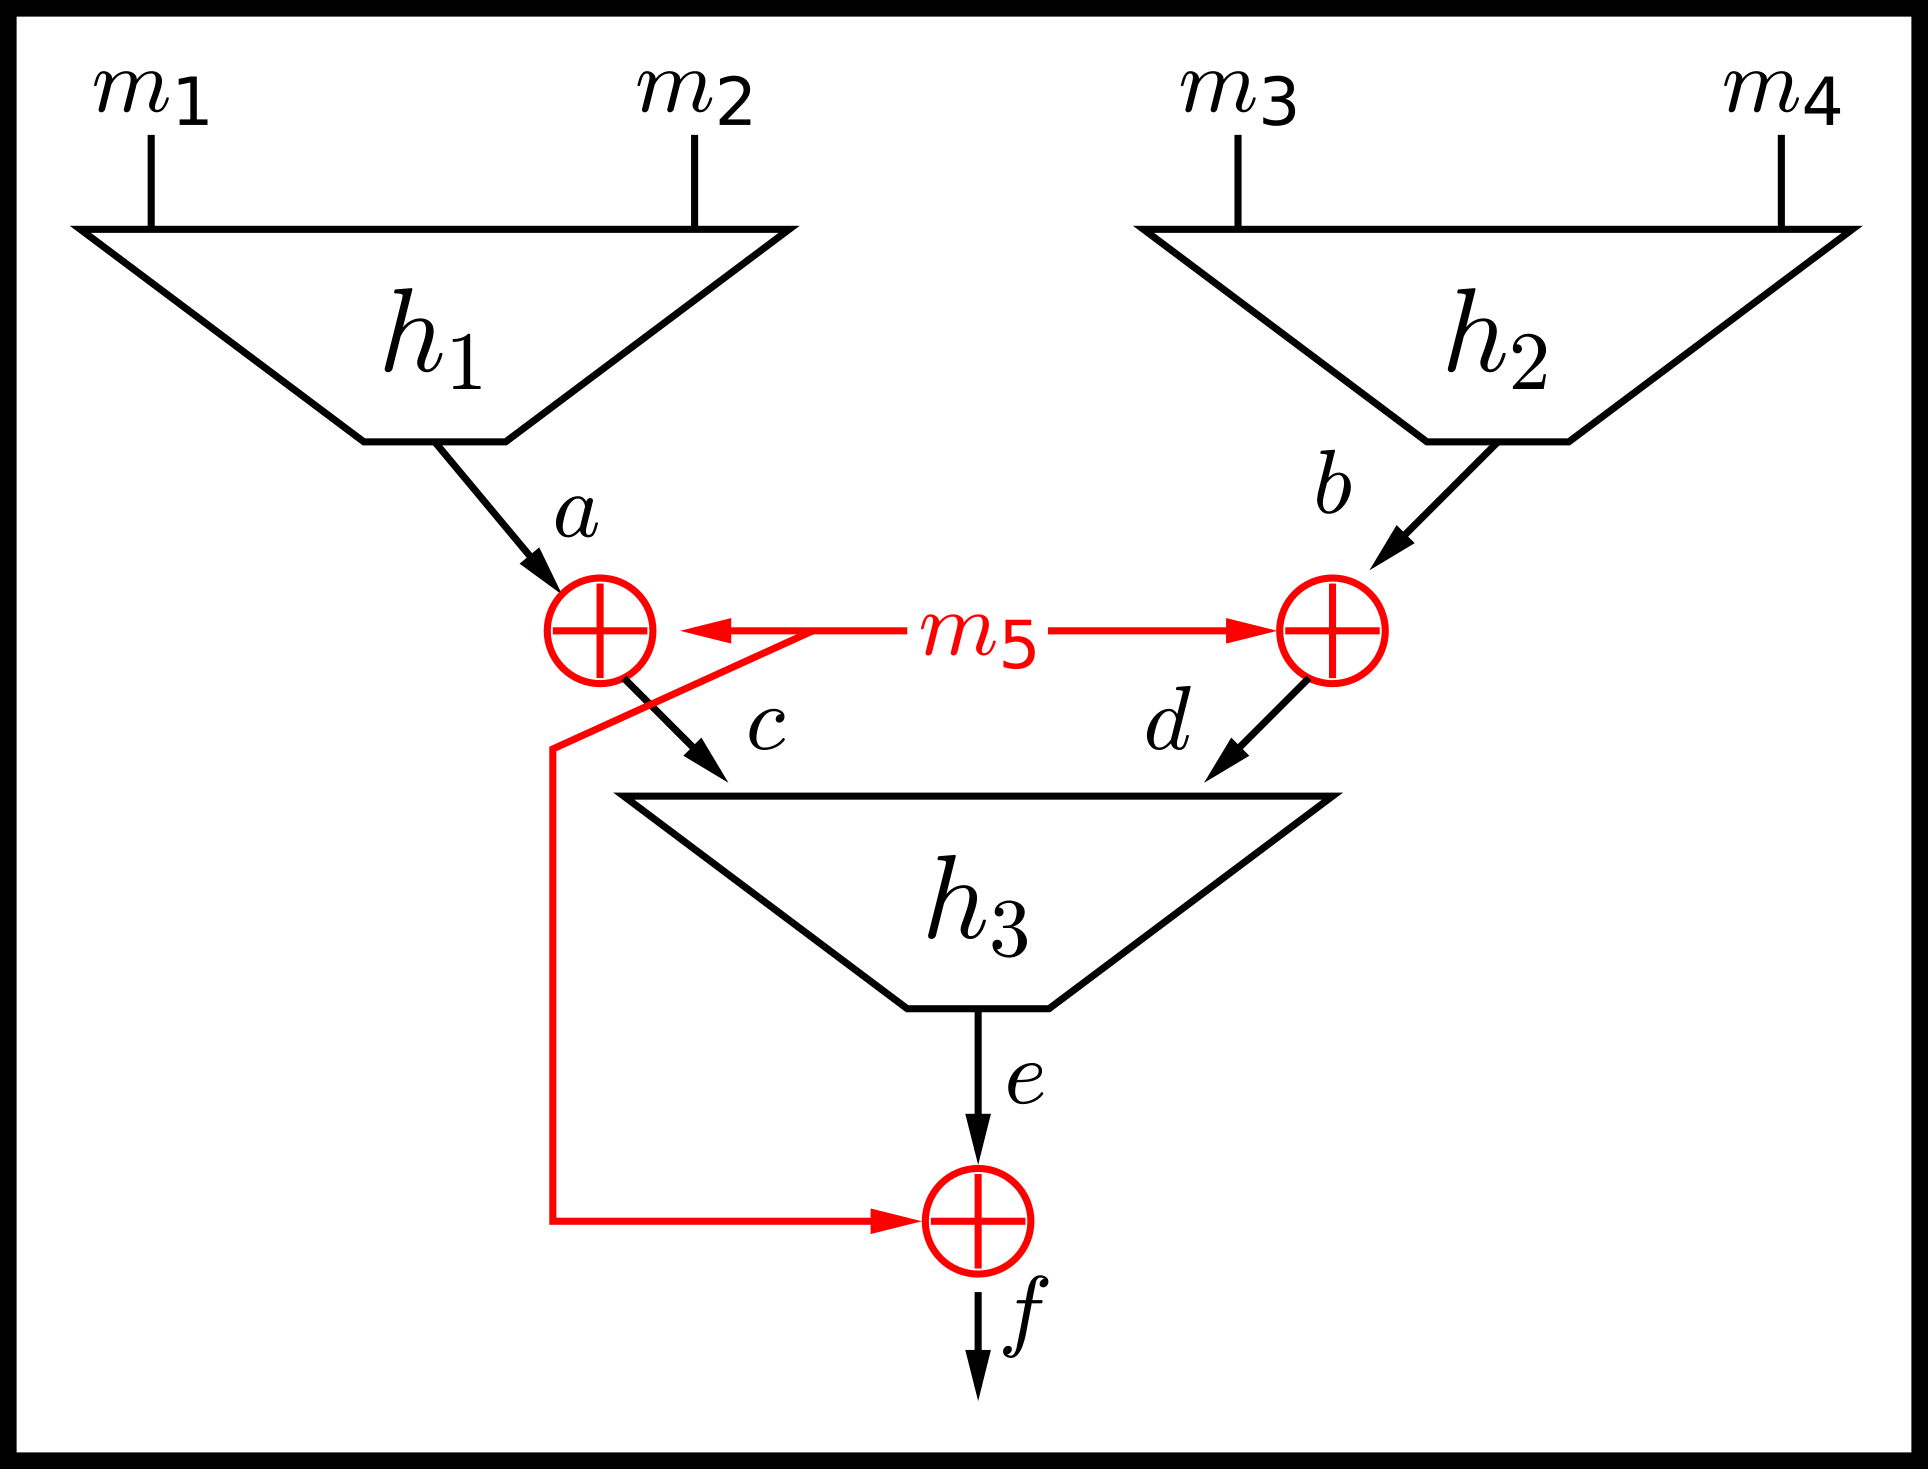
\includegraphics[]{images/Methods/abcd_paperT5_block_depiction.png}
\caption{Modified Merkle tree $T_5(m_1, m_2, m_3, m_4, m_5)$ of height d = 2,   with an extra input $m_5$ for the same 3 hash calls $h_1, h_2, h_3$. In this work, it is referred to as one $T_5$-Block.~\cite{T5_paper}}
\label{img:t5_paper_block_depiction}
\end{figure}

\subsection{T5 Openings}
To calculate the authentication path (see also Section~\ref{sec:mss_sig_gen} ) in one T5-Block, two different approaches \textit{Conservative Opening} and \textit{Aggressive Opening} are shown by Dodis et al.~\cite{T5_paper}. These two versions are depicted in Figure~\ref{img:t5_conserv_aggr_opening}.
The process of calculating an authentication path is here referred to as \textit{opening}. 

\subsubsection{Conservative Opening}
\label{sec:conserv_opening}
Given a node $m_i, i \in \{1,2,3,4\}$, the straightforward way to open the $T_5$-Block is to provide the remaining four nodes $m_{j \neq i}$. This is denoted as Conservative Opening and depicted in Figure~\ref{img:t5_conserv_aggr_opening}: The current node on the path is $m_1$ (colored green), the remaining four nodes (colored red) necessary for the authentication path to open $m_1$ are $m_2, m_3, m_4, m_5$. The functions $h_1, h_2, h_3$ (colored red) have to be calculated. The performance of the Conservative Method is less attractive than of the other methods and even worse than using a standard Merkle Tree: For authenticating one T5-Block, three hash calls and five elements in the authentication path are necessary, see also Table~\ref{table:conserv_opening}. Therefore, this method is not further considered in this work. % reference to authentication method with merkle tree -> #hashcalls, el. in authpath in table

\begin{table}
\centering
\begin{tabular}{l c} 
 \hline\noalign{\smallskip}
 \multicolumn{2}{c}{\textbf{Conservative Opening}} \\
 \hline\noalign{\smallskip}
 \# el. in auth. path & 4 \\
  \# hashcalls verify & 3 \\
 \hline
\end{tabular}
\caption{Performance of calculating the authentication path for one $T_5$-Block with Conservative Opening: The necessary amount of hashcalls and amount of elements in the authentication path are given.}
\label{table:conserv_opening}
\end{table}

\subsubsection{Aggressive Opening}
\label{sec:aggr_opening}
The second version of opening a $T_5$-Block with better performance than Conservative Opening is the Aggressive Opening. The provable security bounds decreases for this method, but the security remains the same under plausible attack scenarios. It is defined as follows: For a given opening node $m_i, i \in \{1,2,3,4,5\}$, the function $open_{aggr}$ returns the authentication path elements for the corresponding $T_5$-Block:

\begin{align}
&open_{aggr}(m_1) = (m_2, m_5, h_2(m_3,m_4) \oplus m_5) = (m_2, m_5, d) \label{eq:aggr_open_m1_example} \\
&open_{aggr}(m_2) = (m_1, m_5, h_2(m_3,m_4) \oplus m_5) = (m_1, m_5, d) \\
&open_{aggr}(m_3) = (m_4, m_5, h_1(m_1, m_2) \oplus m_5) = (m_4, m_5, c) \\ 
&open_{aggr}(m_4) = (m_3, m_5, h_1(m_1, m_2) \oplus m_5) = (m_3, m_5, c) \\ 
&open_{aggr}(m_5) = (m_1, m_2, h_2(m_3, m_4) \oplus m_5) = (m_1, m_2, d) \label{eq:aggr_open_m5_example}
\end{align}
In Figure~\ref{img:t5_conserv_aggr_opening}, Aggressive Opening is depicted as example for opening node $m_1$ (colored green), see Equation~\ref{eq:aggr_open_m1_example}. 
As shown for all opening nodes in Equations~\ref{eq:aggr_open_m1_example}-\ref{eq:aggr_open_m5_example}, with the Aggressive Opening method the authentication path always contains three elements and the verifier needs two hash calls ($h_1$ or $h_2$ respectively and always $h_3$) to calculate the "root" $f$ of one $T_5$-Block, see Table~\ref{table:aggr_opening}.

\begin{table}
\centering
\begin{tabular}{l c} 
 \hline\noalign{\smallskip}
 \multicolumn{2}{c}{\textbf{Aggressive Opening}} \\
 \hline\noalign{\smallskip}
 \# el. in auth. path & 3 \\
 \# hashcalls verify & 2 \\
 \hline
\end{tabular}
\caption{Performance of calculating the authentication path for one $T_5$-Block with Aggressive Opening.}
\label{table:aggr_opening}
\end{table}

\begin{figure}
\centering
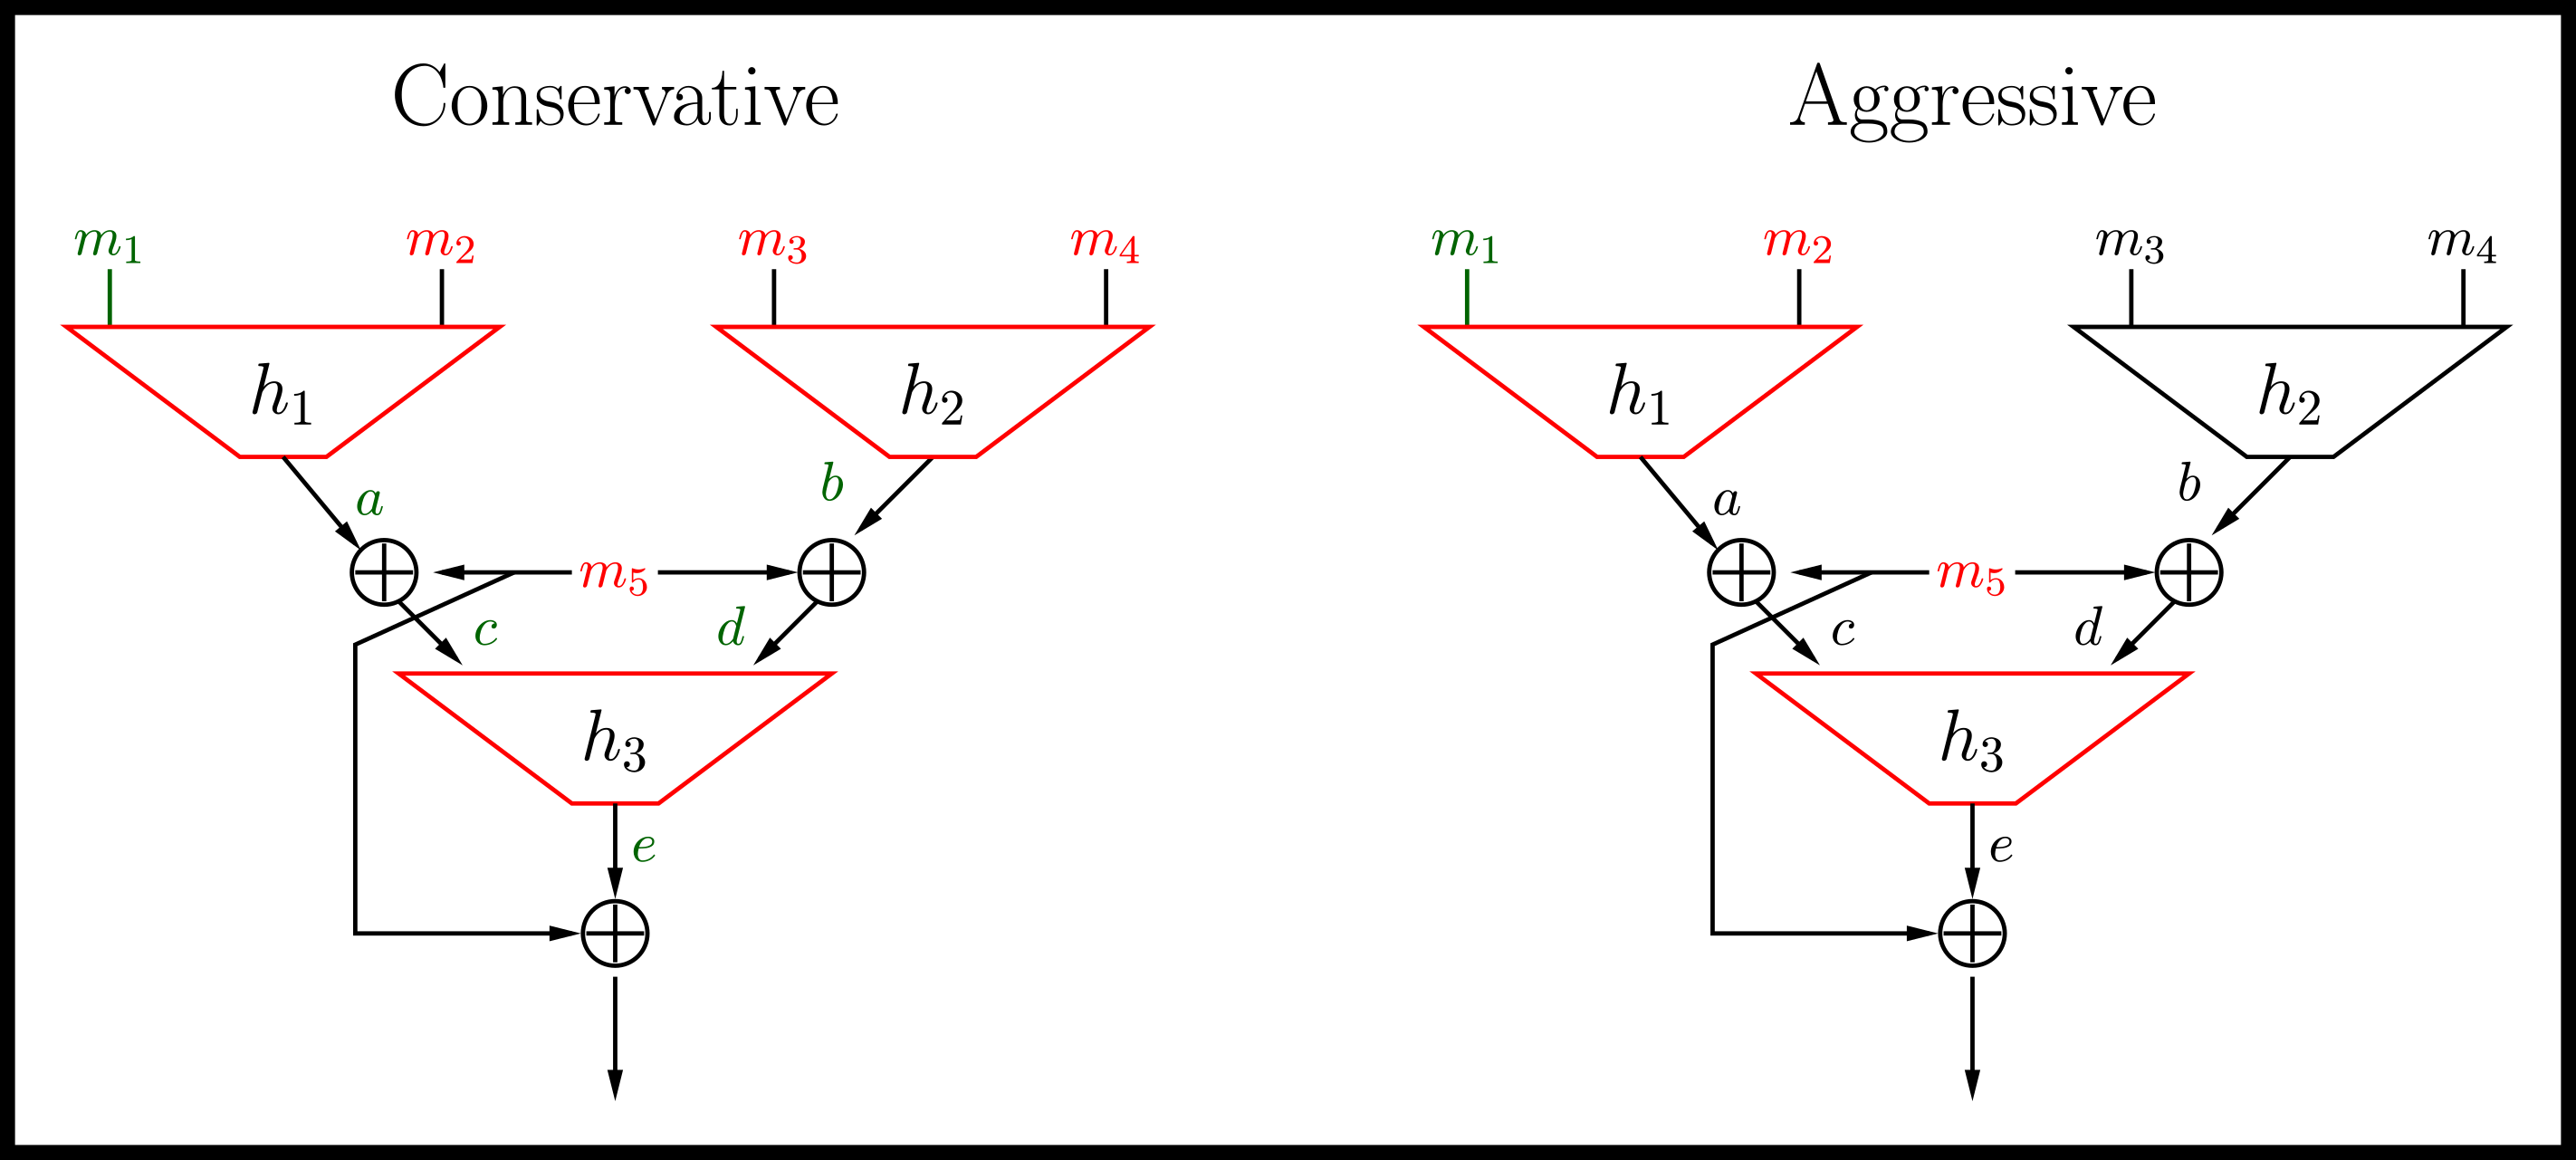
\includegraphics[]{images/Methods/aggr_conserv_opening_T5.png}
\caption{Conservative and Aggressive Opening of one $T_5$-Block. The green variable denotes the opening node, the red nodes are given in the authentication path for this $T_5$-Block. The hash functions denoted in red have to be calculated by the verifier to get the path for this $T_5$-Block.~\cite{T5_paper}}
\label{img:t5_conserv_aggr_opening}
\end{figure}

\subsection{T5 Merkle Tree}
\label{sec:dodis_t5_merkle_tree}
Given the $T_5$-Block construction in Section~\ref{sec:t5_block}, a complete \textit{$T_5$ Merkle Tree}, denoted as \textit{\tftree}, can be built. This is also shown by Dodis et al.~\cite{T5_paper}, see Figure~\ref{img:t5_complete_tree_paper}. Notably, the compression functions $h_1, h_2, h_3$ are the same function, the different indices are used for readability. The performance of the \tftree (including Conservative- and Aggressive Opening variants) in comparison to the standard Merkle Tree is shown in Table~\ref{table:t5_merkletree_dodis_performance}: \textit{Build calls} denote the amount of hash calls necessary for building the whole $T_5$ Merkle Tree, \textit{opening} denotes thee length of the authentication path, \textit{verify} denotes the amount of hash calls needed to build the path (out of the authentication path). \textit{Tree depth} is the amount of layers in the binary Merkle tree compared with the amount of layers in \tftree - this corresponds to the amount of $T_5$ blocks $\times 2$ because one \tfblock corresponds to two Merkle tree layers (see also Figure~\ref{img:t5_paper_block_depiction}).

\begin{table}
\centering
\begin{tabular}{l c c c} 
 \hline\noalign{\smallskip}
 \multicolumn{4}{c}{\textbf{$T_5$ Merkle Tree Performance}} \\
 \hline\noalign{\smallskip}
 & Merkle Tree (standard) & Conserv. Opening &  Aggr. Opening \\
 \hline\noalign{\smallskip}
 build calls$/t$ & 1 & 0.75 & 0.75 \\
 tree depth$/\log_2(t)$ & 1 & 0.86 & 0.86 \\
 verify (hash calls)$/\log_2(t)$ & 1 & 1.29 & 0.86 \\
 opening (length)$/\log_2(t)$ & 1 & 1.72 & 1.29 \\ 
 \hline
\end{tabular}
\caption{Performance of the $T_5$ Merkle Tree with the opening variants Conservative- and Aggressive Opening in comparison to the standard Merkle Tree given by Dodis et al.~\cite{T5_paper}. The variable $t$ denotes the amount of children.}
\label{table:t5_merkletree_dodis_performance}
\end{table}

\begin{figure}
\centering
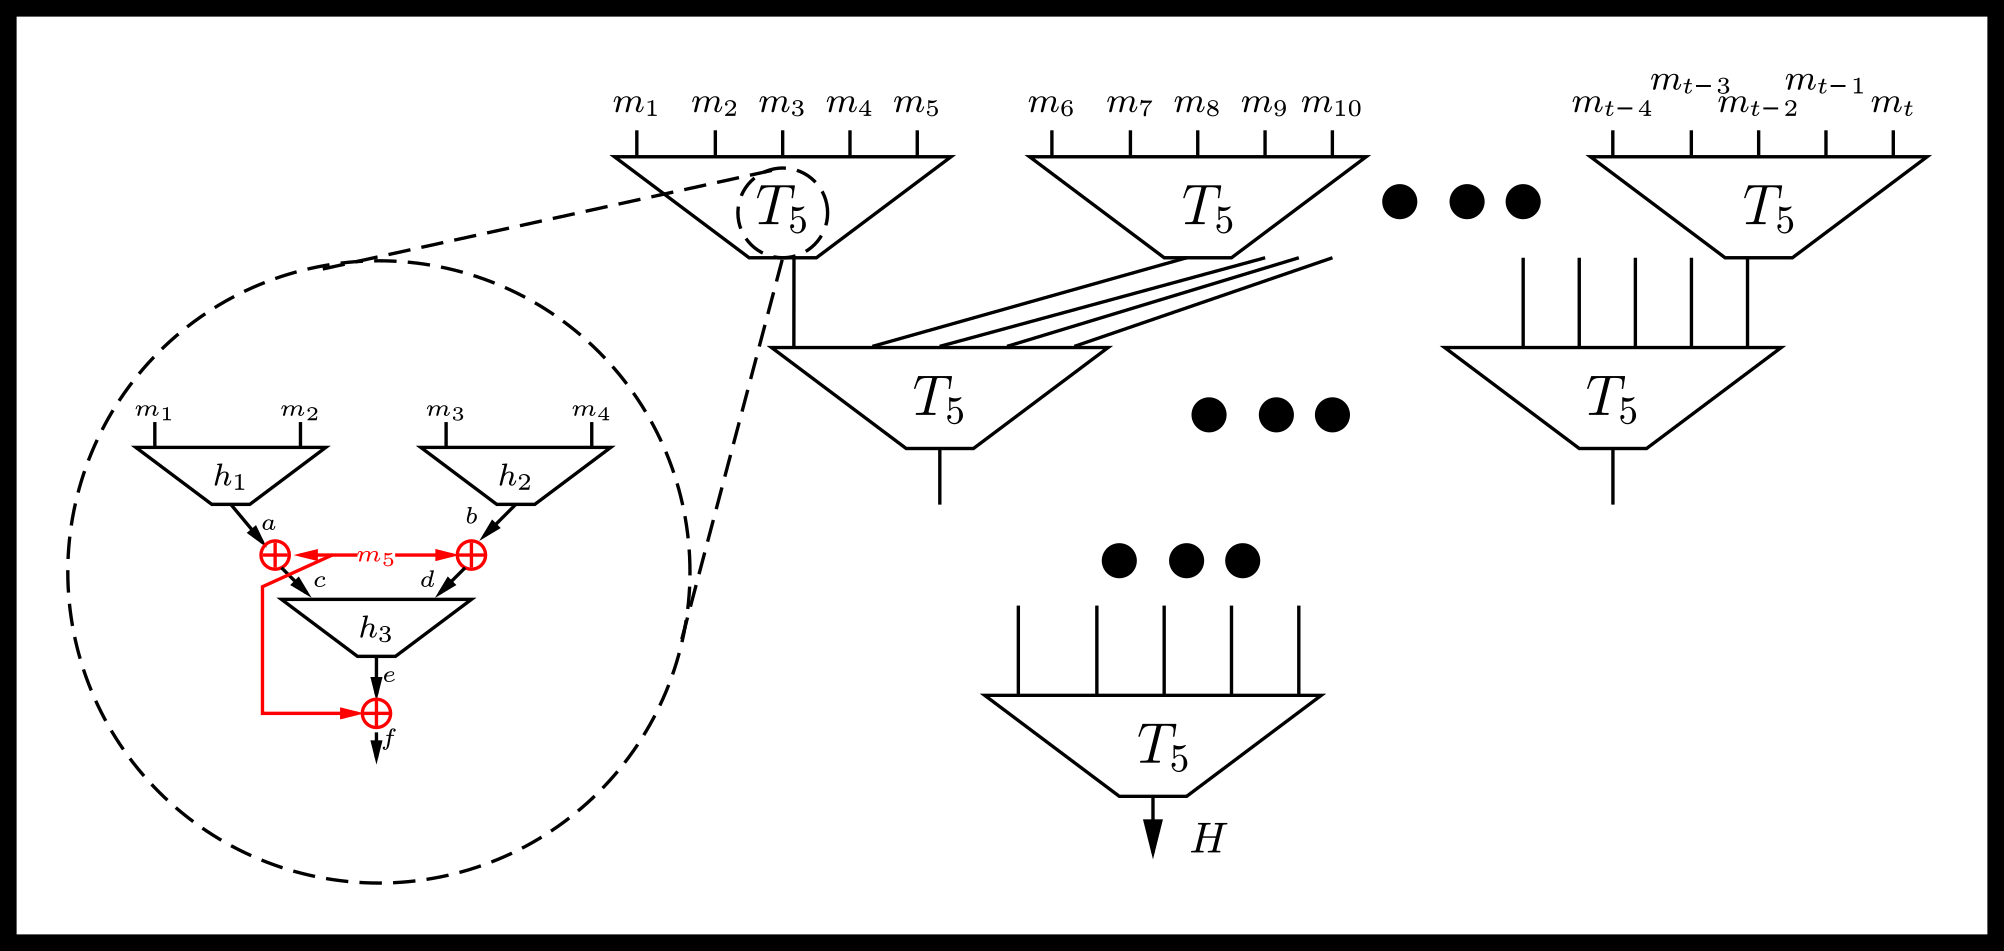
\includegraphics[]{images/Methods/whole_tree_T5_paper.png}
\caption{Construction of a complete $T_5$-Tree consisting of several $T_5$-Blocks~\cite{T5_paper}. The value $H$ denotes the root of the tree.}
\label{img:t5_complete_tree_paper}
\end{figure}

\section{Extended T5 Merkle Tree}
\label{sec:ext_t5_tree} % "my idea"
In this section, the idea of the \tftree is extended by an opening method \textit{More Aggressive Opening}. When implemented in the whole $T_5$~Merkle tree, the tree construction is denoted as \textit{\extree}.
The performance of \extree is compared to \tftree with Aggressive Opening of Dodis et al.~\cite{T5_paper}. There is also a python implementation of \extree as digital signature scheme that contains the steps from key generation to signature verification, see Appendix~\ref{cha:appendix_t5_tree_implementation}.
The parameters used for \extree construction are denoted in Table~\ref{table:t5_ext_parameter}.


\begin{table}
\centering
\begin{tabular}{c l}
 \hline\noalign{\smallskip}
 \multicolumn{2}{c}{\textbf{\extree Parameter}} \\
 symbol & meaning \\
 \hline\noalign{\smallskip} 
 $T$ & height of the tree in $T_5$-Blocks. $T = \log_5(\ell)$ \\
  $\ell$ & amount of leaves. $\ell = 5^T$ \\
 $d$ & height of the tree in actual Merkle nodes. $d = 3T$ \\
 \hline
\end{tabular}
\caption{The parameters of \extree. Notably, one \tfblock contains three Merkle layers, therefore $d=3T$ (see also Figure~\ref{img:t5_paper_block_depiction}).} % explain correlation T, d -> d = 3T really correct? maybe picture of T5Tree+?`
\label{table:t5_ext_parameter}
\end{table}

\subsection{More Aggressive Opening}
\label{sec:more_aggr_opening}
In this work, the new opening method \textit{More Aggressive Opening} is proposed, see Figure~\ref{img:t5_more_aggr_opening}. It has better overall performance than Conservative- and Aggressive Opening (see Section~\ref{sec:aggr_opening} and \ref{sec:conserv_opening}) for the signing and verifying process, see Table~\ref{table:more_aggr_opening}. But notably, the length of the authentication path is \textbf{not} constant.

\subsubsection{Signature Generation: \texorpdfstring{\tfblock}{T5-Block}}
When calculating the authentication path (generating the signature) for one \tfblock, two cases distinguished:

\begin{itemize}
\label{list:case1_case_2}
\item \textbf{Case~1}: The possible opening nodes are $m_i, i \in \{1,2,3,4\}$. For a given opening node $m_i$, the function $open_{aggr+}$ returns the authentication path for the corresponding \tfblock:
\begin{align}
open_{aggr+}(m_1) = (m_2, m_5, h_2(m_3, m_4)) = (m_2, m_5, b) = A_{m_1+} \label{eq:more_aggr_m1_example} \\
open_{aggr+}(m_2) = (m_1, m_5, h_2(m_3, m_4)) = (m_1, m_5, b) = A_{m_2+} \\
open_{aggr+}(m_3) = (m_4, m_5, h_1(m_1, m_2)) = (m_4, m_5, a) = A_{m_3+} \\
open_{aggr+}(m_4) = (m_3, m_5, h_1(m_1, m_2)) = (m_3, m_5, a) = A_{m_4+} \label{eq:more_aggr_m4_example}
\end{align} 
An example of $m_1$ as opening node is depicted on the left side of Figure~\ref{img:t5_more_aggr_opening}: The signer is putting the elements $m_2, m_5, b$ in the authentication path (see Equation~\ref{eq:more_aggr_m1_example}). The verifier needs two hash calls ($h_1, h_3$) to calculate the path to the root $f$.
Therefore, the authentication path has always three elements and the verifier always needs two hash calls to calculate the path to the root of one \tfblock for case~1, see also Table~\ref{table:more_aggr_opening}.

\item \textbf{Case~2}: The opening node is $m_5$. This case is depicted on the right side of Figure~\ref{img:t5_more_aggr_opening}. For $m_5$ as opening node, the function $open_{aggr+}$ returns the authentication path for the corresponding \tfblock:
\begin{equation}
\label{eq:more_aggr_opening_m5_example}
open_{aggr+}(m_5) = (h_1(m_1, m_2), h_2(m_3, m_4)) = (a, b) = A_{m_5+}
\end{equation}
An example of $m_5$ as opening node is depicted on the right side of Figure~\ref{img:t5_more_aggr_opening}: The signer is putting the elements $a, b$ in the authentication path (see Equation~\ref{eq:more_aggr_opening_m5_example}). The verifier needs one hash call $h_3$ to calculate the path to the root $f$.
Therefore, the authentication path has always two elements and the verifier always needs one hash call to calculate the path to the root for one \tfblock for case~2, see also Table~\ref{table:more_aggr_opening}.
\end{itemize} 

\begin{figure}
\centering
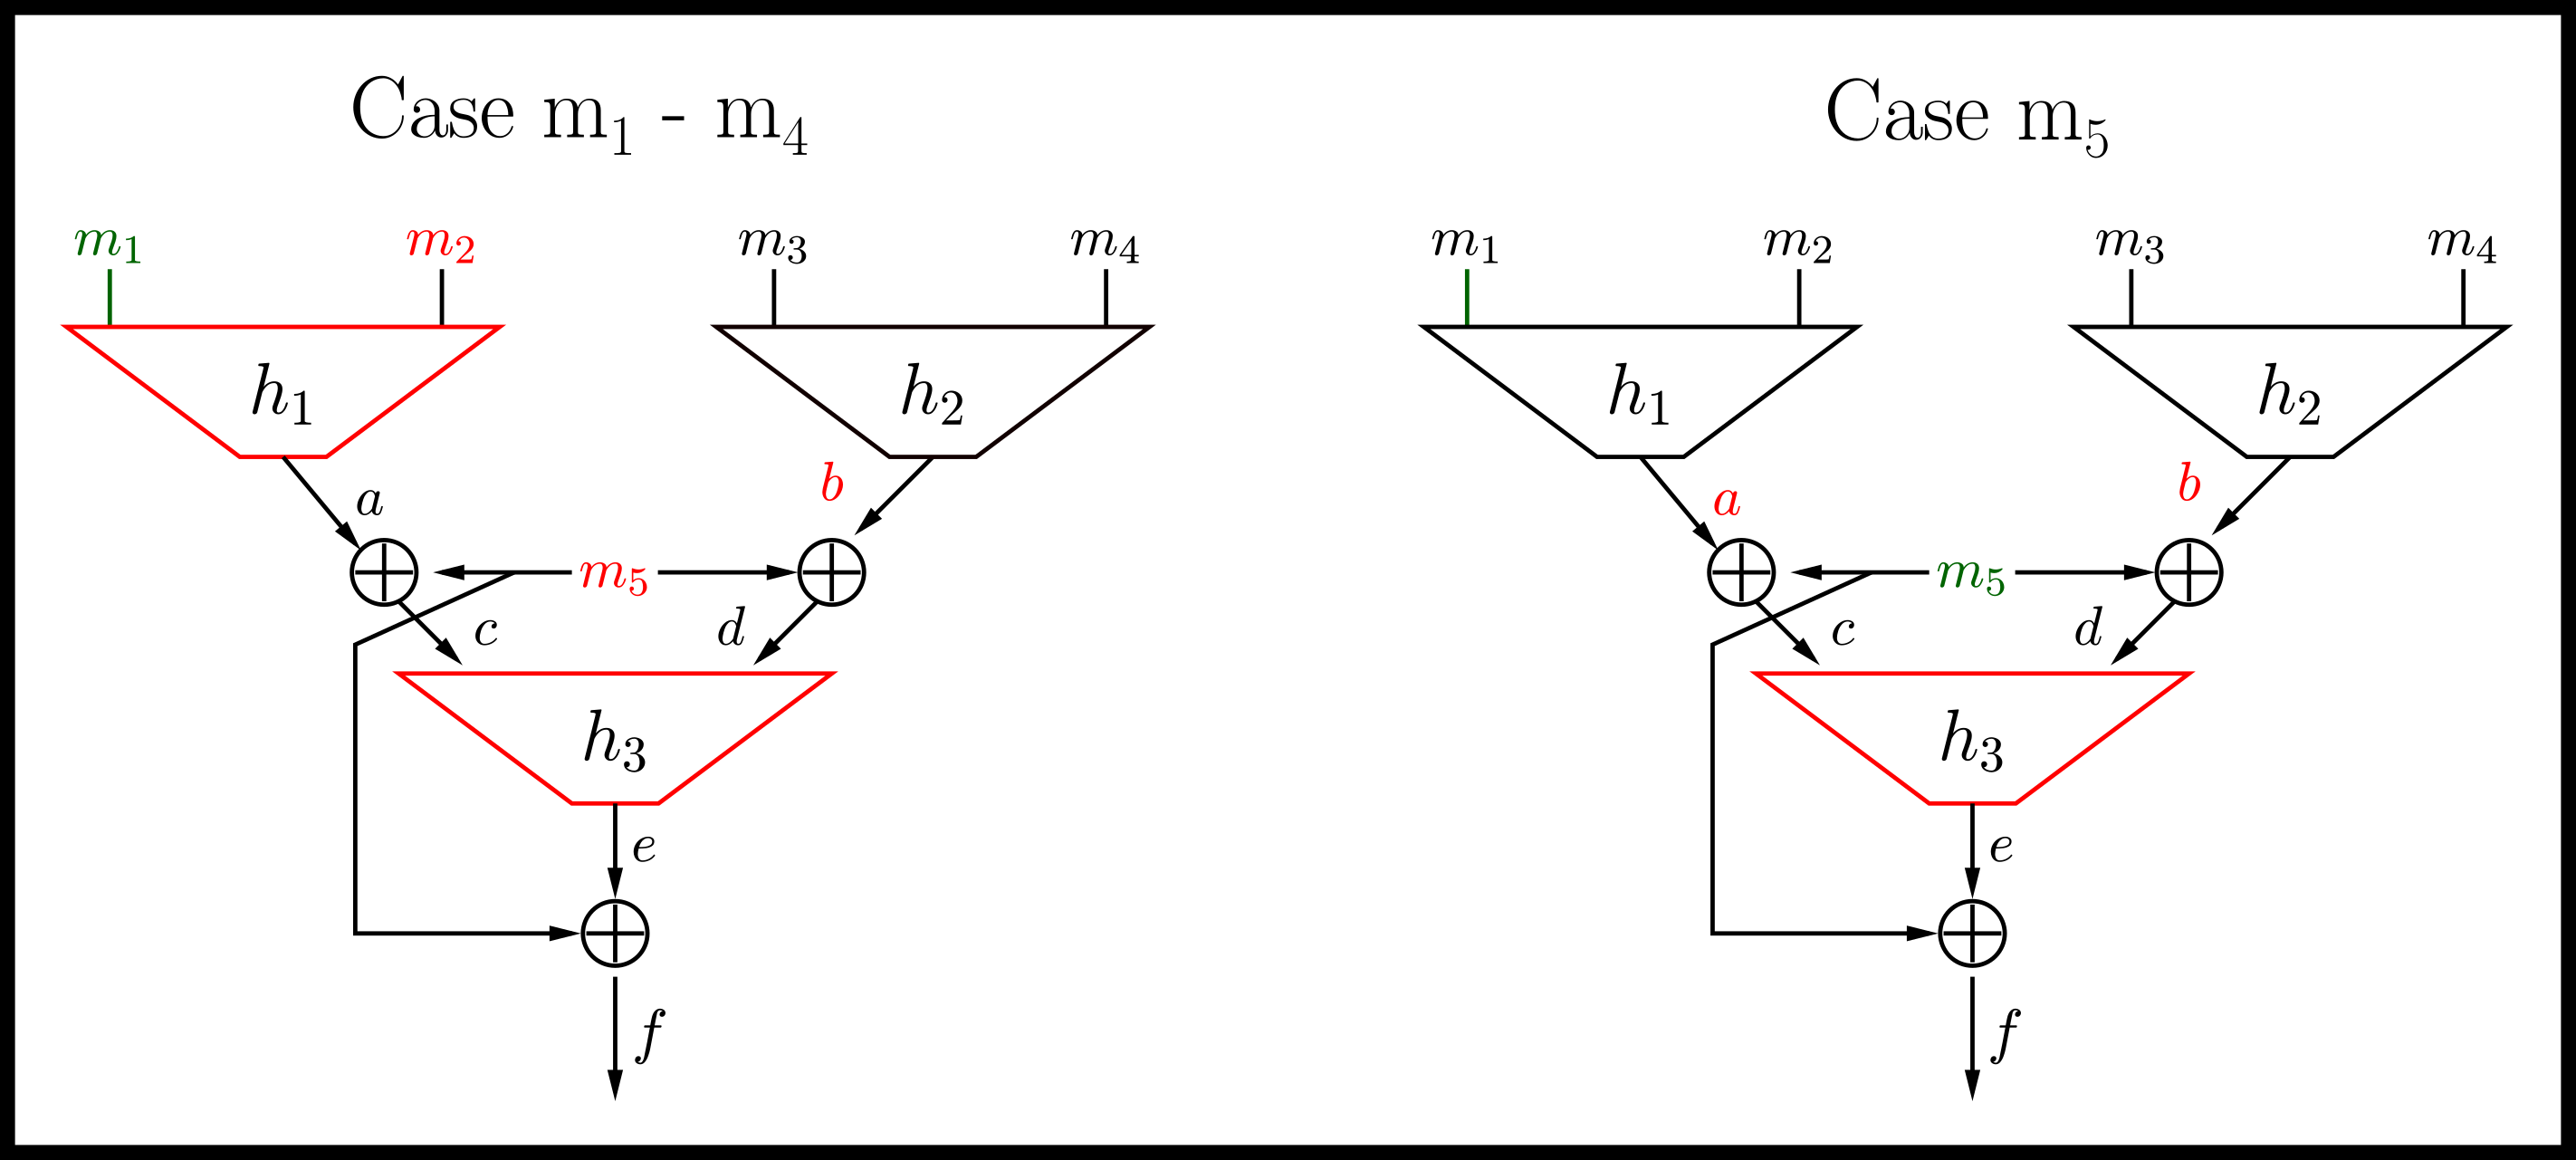
\includegraphics[]{images/Methods/more_aggr_opening.png}
\caption{More Aggressive Opening for one \tfblock, with case differentiation. The green variable denotes the opening node, the red nodes are given in the authentication path the respective \tfblock. The hash functions denoted in red have to be calculated by the verifier to get the path for this \tfblock.}
\label{img:t5_more_aggr_opening}
\end{figure}

\begin{table}
\centering
\begin{tabular}{l c c} 
 \hline\noalign{\smallskip}
 \multicolumn{3}{c}{\textbf{More Aggressive Opening}} \\
 \hline\noalign{\smallskip}
 & case 1: $m_i, i \in \{1,2,3,4\}$ & case 2: $m_5$ \\
 \# el. in auth. path & 3 & 2 \\
 \# hashcalls verify & 2 & 1 \\
 \hline
\end{tabular}
\caption{Performance of calculating the authentication path and amount of elements in the authentication path for More Aggressive Opening. The case~1 with $m_i, i \in \{1,2,3,4\}$ as possible opening/path nodes and case~2 with $m_5$ as opening/path node are shown.}
\label{table:more_aggr_opening}
\end{table}

\subsubsection{Signature Verification: \texorpdfstring{\tfblock}{T5-Block}}
When calculating the path (verifying the signature) for one \tfblock, the same two cases as for signature generation are distinguished (see Equation~\ref{eq:more_aggr_m1_example}-\ref{eq:more_aggr_m4_example} and Equation~\ref{eq:more_aggr_opening_m5_example} respectively). For an explanatory depiction of the two cases, see Figure~\ref{img:t5_more_aggr_opening}.

\begin{itemize}
\item \textbf{Case~1}: The possible leaves of the \tfblock, for which a path to the root $f$ will be calculated by the verifier, are $m_i, i \in \{1,2,3,4\}$. For leaf $m_i$ and the corresponding authentication path $A_{m_i+}$ (given by the signer, see Equation~\ref{eq:more_aggr_m1_example}-\ref{eq:more_aggr_m4_example}), the function $path(m_i,A_{m_i+})$ returns the root $f$ for the corresponding \tfblock:

\begin{align}
&path(m_1, A_{m_1+}) = path(m_1, (m_2, m_5, b)) = h_3(h_1(m_1, m_2) \oplus m_5, b \oplus m_5) \oplus m_5 = f \label{eq:more_aggr_path_m1}\\
&path(m_2, A_{m_2+}) = path(m_2, (m_1, m_5, b)) = h_3(h_1(m_1, m_2) \oplus m_5, b \oplus m_5) \oplus m_5 = f\\
&path(m_3, A_{m_3+}) = path(m_3, (m_4, m_5, a)) = h_3(a \oplus m_5, h_2(m_3, m_4) \oplus m_5) \oplus m_5 = f \\
&path(m_4, A_{m_4+}) = path(m_4, (m_3, m_5, a)) = h_3(a \oplus m_5, h_2(m_3, m_4) \oplus m_5) \oplus m_5 = f \label{eq:more_aggr_path_m4}
\end{align}

\item \textbf{Case~2}: The path $f$ needs to be calculated for $m_5$ as given "leaf" of the \tfblock. Given $m_5$ and the corresponding authentication path $A_{m_5+}$ (given by the signer, see Equation~\ref{eq:more_aggr_opening_m5_example}) is calculated by $path(m_5, A_{m_5+})$:
\begin{equation}
\label{eq:more_aggr_path_m5}
path(m_5, A_{m_5+}) =  path(m_5, (a,b)) = h_3(a \oplus m_5, b \oplus m_5) \oplus m_5 = f
\end{equation}
\end{itemize}

The process of tree generation, signing and verifying using Aggressive Opening in the \extree is shown in the following section. 


\subsection{\texorpdfstring{\extree}{Ext. T5-Tree} Generation}
The \extree Generation works like tree generation for the \tftree, see Section~\ref{sec:dodis_t5_merkle_tree}, Section~\ref{cha:mss_keygen} and Figure~\ref{img:t5_complete_tree_paper}. The implementation of the \extree construction in Python is shown in Appendix~\ref{cha:appendix_t5_tree_implementation}.
% maybe pseudocode but too complex -> just read appendix
% 
The performance equations for building an \extree are derived as follows (see also Table~\ref{table:t5_ext_parameter}). the total amount of \tfblocks in one \extree is:
\begin{equation}
\text{\#\tfblocks} = \sum_{i=0}^{T-1} 5^i
\end{equation} 
For one \tfblock, three hash calls are necessary (see Section~\ref{sec:t5_block}). Therefore, the total amount of hash calls for building \extree based on $T$ is:\\
\begin{equation}
\text{\# hash calls tree gen. (depending on $T$)} = 3 \cdot \sum_{i=0}^{T-1} 5^i
\end{equation}
To get the hash calls for tree generation based on the leaves $\ell$, $T$ is substituted by $\log_5(\ell)$.
\begin{equation}
\text{\# hash calls tree gen. (depending on $\ell$)}=3 \cdot \sum_{i=0}^{\log_5(\ell)-1} 5^i = 3 \cdot \sum_{i=0}^{\frac{\log(\ell)}{\log(5)}-1} 5^i = \frac{3}{4} (\ell-1)
\end{equation}

\subsection{\texorpdfstring{\extree}{Ext. T5-Tree} Signature Generation}
The signature generation for \extree works as follows: After calculating the complete \extree, the signer first calculates the $T_5$-Path (see also line~17, \mintinline{python}{def calc_t5_path}~($\cdots$) in Appendix~\ref{cha:appendix_t5_tree_implementation}).
Now, the signer calculates the authentication path out of the $T_5$-Path (see also line~167, \mintinline{python}{def calc_auth_path}~($\cdots$) in Appendix~\ref{cha:appendix_t5_tree_implementation} and Section~\ref{sec:mss_sig_gen}).

For this version of the \extree, it is assumed the signer saves the whole tree  after key generation. Therefore, no additional hash calls are necessary for generating the authentication path. % maybe insert #hashcalls for winternitz ots generation
As \extree uses More Aggressive Opening, the length of the authentication path differs on the case, see Section~\ref{sec:more_aggr_opening}.
For \textbf{case~1}, there are always three elements in the authentication path for one \tfblock, see Equation~\ref{eq:more_aggr_m1_example}-\ref{eq:more_aggr_m4_example} and Table~\ref{table:more_aggr_opening}.
For \textbf{case~2}, there are always two elements in the authentication path, see Equation~\ref{eq:more_aggr_opening_m5_example}. For of all signatures used in one \extree, the average of \textbf{case~1} is $\frac{4}{5}$ , whereas the average \textbf{case~2} is $\frac{1}{5}$.
Therefore, the average amount of elements in the authentication path is calculated as follows:
\begin{equation}
\label{eq:more_aggr_len_authpath}
\text{\# elements auth.path (average)} = 3 \cdot \frac{4}{5} + 2 \cdot \frac{1}{5} = 2.8
\end{equation}

\subsection{\texorpdfstring{\extree}{Ext. T5-Tree} Signature Verification}
After receiving the authentication path by the signer, the verifier calculates the path through the \extree to its root (see also line~28, \mintinline{python}{def calc_path_verifier}~($\cdots$) in Appendix~\ref{cha:appendix_t5_tree_implementation}). The verifier compares the calculated root with the public key of the signer, if they match, the signature is valid (see Section~\ref{sec:mss_sign_verif}).

With the More Aggressive opening variant used in the \extree, calculating the path for \textbf{case~1} needs two hash calls (see Equation~\ref{eq:more_aggr_path_m1}-\ref{eq:more_aggr_path_m4}) and calculating it for \textbf{case~2} needs one hash call (see Equation~\ref{eq:more_aggr_path_m5}). The average of each case over of all signature verifications (for one \extree), is $\frac{4}{5}$ for\ \textbf{case~1} and $\frac{1}{5}$ for \textbf{case~2}. Therefore, the average amount of hash calls necessary for calculating the root $f$ of the \extree is calculated as follows:

\begin{equation}
\text{\# hash calls path calculation} = \frac{4}{5} \cdot 2 + \frac{1}{5} = 1.8
\end{equation}


\chapter{Evaluation}
\label{cha:evaluation}

In this chapter, the performance results of the different methods (see Chapter~\ref{cha:methods}) are shown.

\section{NIST Parameter}


\begin{table}
\centering
\begin{tabular}{l c c l l} 
 \hline\noalign{\smallskip}
 \textbf{LMS Parameter Sets} & \textbf{Numeric Identifier} & \textbf{$m$} & \textbf{$h$} & $\ell$ \\
 \hline\noalign{\smallskip}
 LMS\_SHA256\_M32\_H5 & 0x00000005  & 32 & 5 & $32$ \\
 LMS\_SHA256\_M32\_H10 & 0x00000006  & 32 & 10 & $1024$ \\
 LMS\_SHA256\_M32\_H15 & 0x00000007  & 32 & 15 & $32768$ \\
 LMS\_SHA256\_M32\_H20 & 0x00000008  & 32 & 20 & $1048576$ \\
 LMS\_SHA256\_M32\_H35 & 0x00000009  & 32 & 25 & $33554432$ \\
 \hline\noalign{\smallskip}
 \end{tabular}
\caption{NIST LMS parameter sets for SHA-256~\cite{stateful_hashbased_sign_schemes_NIST_2020}. The variable $m$ denotes the number of bytes associated with each node in the LMS Merkle tree (used by LMS), the parameter $h$ denotes the height and $\ell = 2^h$ denotes the amount of children of the Merkle tree.} % insert reference to LMS section here
\label{table:nist_param_lms}
\end{table}

% table with formulas
\begin{table}
\centering
\begin{tabular}{l c c c} 
 \hline\noalign{\smallskip}
 \multicolumn{4}{c}{\textbf{Performance in General}} \\
 \hline\noalign{\smallskip}
 & & \textbf{\tftree} & \textbf{\extree} \\
 \noalign{\smallskip}
  & \textbf{Merkle Tree (standard)} & Aggr. & More Aggr. \\
 \hline\noalign{\smallskip}
 \# hash calls keygen & $\ell-1$ & \multicolumn{2}{c}{$\frac{3}{4}\ell$} \\
 \# saved nodes (whole tree) & $2\ell-1$ & \multicolumn{2}{c}{$10\ell-1$} \\ % check if really true
 \# hash calls sign (authpath generation) & $\emptyset$ & \multicolumn{2}{c}{$\emptyset$} \\
 \# el. in authpath generation & $\log_2(\ell)$ & $3\log_5(\ell)$ & $2.8\log_5(\ell)$\\
 \# hash calls path calculation & $\log_2(\ell)$ & $3\log_5(\ell)$ & $1.8\log_5(\ell)$\\ 
 \hline
\end{tabular}
\caption{Performance of the the standard Merkle tree and \extree with the opening variants Aggressive Opening (Aggr.) and More Aggressive Opening (More Aggr.), see Sections~\ref{sec:more_aggr_opening} and ~\ref{sec:aggr_opening} respectively. The variable $\ell$ denotes the amount of leaves.}
\label{table:general_formulas_t5_merkle}
\end{table}

% \section{Discussion}

% \section{Future Work}
% idea for xmss, not only calculating the speedup but also concept
\chapter{Conclusion}
\label{cha:conclusion}
In this work, the goal was to analyze quantum-secure hash-based signature systems (HBS) in detail and to find opportunities for performance improvements and implementing them. 
To solve this task, the T$_5$-Method of Dodis et al.~\cite{T5_paper} is used to introduce the tree concepts \tftree (see Section~\ref{sec:dodis_t5_merkle_tree}) and \extree (see Section~\ref{sec:ext_t5_tree}). 
It is shown that the Merkle Tree in LMS (and potentially XMSS and other signature schemes) can be substituted with these alternate tree concepts.

\section{Discussion}
Both T$_5$ tree concepts outperform the classical Merkle Tree in key generation and verification time when used in LMS. \tftree needs $25\%$ fewer hash calls for key generation and $14\%$ fewer hash calls for verification. \extree also reduces the amount of hash calls for key generation by $25\%$ and achieves the best result for verification time with $22\%$ fewer hash calls.
The length of the authentication path increases for \tftree and \extree by $29\%$ and $20\%$ respectively. The length of the authentication path for \extree is not constant. If a constant length is needed, \tftree is the better choice though \extree has better performance.
Notably, key generation time increases exponentially, whereas verification time and length of the authentication path increases linear (dependent on the tree height). Therefore, the worse performance for authentication path length does not have as much impact. 
% NIST param set LMS (notably, leaf generation/WOTS not taken into account)

\section{Future Work}
XMSS was inspected in detail in this work, but inserting the T$_5$ trees into XMSS is still an open task. As XMSS uses bitmasks in its Merkle Tree, the T$_5$ tree concepts would need to be adapted. One idea how to achieve this, is using the bitmasks as node $m_5$ for one \tftree, as the bitmasks in XMSS are also inserted to the tree via XOR operations.
% idea
Another idea worth exploring is adapting \tftree and \extree for not using each leaf as a one-time key (i.e. not making them perfect trees). This would lead to a broader variety of possible one-time keys: With the current concept, the possible amount of one-time keys has to be a power of five. This could be achieved by not calculating each sub-tree of a \tftree, but only parts of it.
% idea
To distribute the time and space effort between signer and verifier, the signing and authentication operations for one \tfblock could be adapted: 
For example if the signer has more computing resources, the signer could directly calculate $c,d$ (of one \tfblock) instead of $a,b$ (see Figure~\ref{img:t5_more_aggr_opening}). As a result, the signer computes the two XOR computations during signing instead of the verifier during verification.
% idea
Finally, speeding up a stateless HBS with the T$_5$ methods is also achievable: For SPHINCS+ exists an instantiation denoted as SPHINCS+-simple~\cite{sphincs+_submussion_nist_round3}, which contains a standard Merkle Tree. This makes inserting \tftree and \extree easily possible.


\appendix 
\chapter{Python Implementation: Extended T5 Tree}
\label{cha:appendix_t5_tree_implementation}
The python implementation of \textit{\extree} (see also Section~\ref{sec:ext_t5_tree}) is shown here.

\lstinputlisting[language=Python, breaklines=true]{scripts/T5Tree.py}


\chapter{Python Implementation: Performance Evaluation}
\label{cha:appendix2_performance_calc}

The performance of the tree concepts Merkle Tree (see Section~\ref{sec:mss}), \tftree (see Section~\ref{sec:dodis_t5_merkle_tree}) and \extree (see Section~\ref{sec:ext_t5_tree}) for Chapter~\ref{cha:evaluation} is calculated with the following python script \mintinline{python}{performance_evaluation.py}:

\inputminted[breaklines,linenos]{python}{scripts/performance_evaluation.py}

\bibliography{bibliography}
\bibliographystyle{IEEEtran}

\end{document}
